\documentclass{article}
\usepackage{graphicx} % Required for inserting images
\usepackage{fancyhdr} % Required for header and footer configuration
\usepackage[a4paper, margin=2.5cm, left=1.5cm, right=1.5cm, bottom=4cm]{geometry} % Required for setting page margins
\usepackage[T1]{fontenc}
\usepackage[default,oldstyle,scale=1]{opensans} % Utilizzo del font Open Sans
\usepackage{lipsum}
\usepackage{makeidx}
\usepackage{booktabs}
\usepackage{tabularray}
\usepackage[colorlinks=true, linkcolor=black, urlcolor=blue, citecolor=blue]{hyperref}
\usepackage{tabularx}
\usepackage{makecell}
\usepackage{enumitem} % Pacchetto per la personalizzazione degli elenchi
\usepackage{booktabs}

% Configure header and footer for the first page
\fancypagestyle{firstpage}{
    \fancyhf{} % Clear header and footer
    \renewcommand{\headrulewidth}{0pt} % Remove header rule line
    \lhead{} % Header on the left
    \chead{} % Header in the center
    \rhead{} % Header on the right
    \lfoot{} % Footer on the left
    \cfoot{\vspace{5pt}\\\hrulefill\\\vspace{10pt}\textbf{BeeLive}\\Gruppo 21} % Footer in the center
    \rfoot{\vspace{32.5pt}\\\thepage} % Footer on the right
}

% Configure header and footer for non-plain pages (second page onwards)
\fancypagestyle{nonplain}{
    \fancyhf{} % Clear header and footer
    \lhead{} % Header on the left
    \chead{} % Header in the center
    \rhead{
\includegraphics[width=2cm]{Images/BeeLive-Logo.png}\\\vspace{2pt}} % Header on the right
    \lfoot{} % Footer on the left
    \cfoot{\vspace{5pt}\\\hrulefill\\\vspace{10pt}\textbf{BeeLive}\\Gruppo 21} % Footer in the center
    \rfoot{\vspace{32.5pt}\\\thepage} % Footer on the right
}

% Adjust vertical space between header and text                                    
\setlength{\headsep}{65pt} 
% Adjust vertical space between text and footer
\setlength{\footskip}{0pt} 

\title{
\includegraphics[width=0.75\textwidth]{Images/BeeLive-Logo.png}\\\vspace{100pt}
\LARGE{\textbf{BeeLive\\Deliverable 1}}}
\author{Gruppo 21:\\
Cipriani Pietro, 226959\\
Orlando Dennis, 227688\\
Ziviani Elia, 228172}
\date{28 Marzo 2024}

\makeindex % Indica che vogliamo creare un indice

\begin{document}

\maketitle
\thispagestyle{firstpage} % Apply firstpage style to the first page
\clearpage

\pagestyle{nonplain} % Apply non-plain style to subsequent pages

\renewcommand{\contentsname}{Indice}
\tableofcontents

\clearpage
\section{Introduzione}
\index{Introduzione} % Aggiunge una voce all'indice

La Municipalità di Trento, in collaborazione con l'Università, ha richiesto che come oggetto di valutazione del corso di \textit{Ingegneria del Software} ideassimo un progetto a tema "Ideare la Trento del futuro".\\
Non sono state date molte altre informazioni o suggerimenti, in modo che il processo di design thinking non fosse contaminato da schemi mentali, limitazioni o idee precedenti. \\
\\
Questo documento è il primo "deliverable" di \textit{BeeLive}, i.e. il progetto da noi proposto per affrontare la suddetta consegna. \\
\\
Un primo processo di brainstorming ci ha permesso di notare come a Trento risulti difficile reperire informazioni riguardanti alcuni eventi, in particolare quelli che influenzano la viabilità stradale. Le informazioni disponibili sono principalmente testuali e richiedono un impegno attivo da parte dei cittadini per essere trovate.
Ciò causa una generale difficoltà nel reperire tali informazioni, aggravato dal fatto che, attualmente, manca un sistema di notifica automatica per tali modifiche.\\
\\
\textit{BeeLive} è una soluzione a questo problema. 

\clearpage

\section{Obiettivi e descrizione dell'applicativo}
\index{Obiettivi e descrizione dell'applicativo}

L'obiettivo che si ripropone questo applicativo è di risolvere i problemi precedentemente menzionati attraverso l'implementazione dei seguenti punti:\\
1. sviluppare un sistema informativo che consenta ai cittadini di accedere rapidamente, intuitivamente e sopratutto \textbf{visivamente} a tutte le variazioni della viabilità, all'interno del comune di Trento\\
\label{Accesso alle notizie}
2. Informare attivamente gli utenti di eventuali modifiche alla viabilità, con particolare attenzione agli eventi che potrebbero colpirli direttamente\\ % l'ho tenuto generale
\label{Informare i cittadini}
\\
Il primo punto prevede lo sviluppo di un sistema informativo che mostri ai cittadini una rappresentazione grafica delle zone interessate da determinati eventi, con focus particolare per le zone coinvolte in eventuali modifiche alla viabilità. \\
\label{Visualizzazione degli eventi}
Il secondo punto prevede la creazione di un sistema di notifiche push, associato al suddetto applicativo mobile, che permetta di notificare attivamente gli utenti di eventuali eventi e modifiche alla viabilità.\\
\label{Notifiche push}
Prevediamo di sviluppare un sistema per cui gli utenti possano impostare dei percorsi abituali in modo che, all'insorgere di un evento che vada a colpire un punto qualunque di tale percorso, l'utente ne sia avvisato. \\
\label{Percorsi abituali}
Prevediamo di dar voce agli interessi individuali di ogni utente, in modo che essi possano indicare delle preferenze per determinate notifiche rispetto ad altre. % molto vago, di proposito
\\
\\
Saranno sviluppati due ambienti distinti: Uno riservato all'amministrazione e uno accessibile ai cittadini.\\
Il primo ambiente consentirà all'amministrazione di inserire e modificare le informazioni sulle variazioni della viabilità attraverso un'interfaccia grafica intuitiva e compatibile con gli standard per la visualizzazione dei dati su mappa.\\
\label{Gestione degli eventi}
Il secondo sarà rappresentato dall'applicativo mobile installabile sui dispositivi dei cittadini, che come precedentemente menzionato consentirà loro di visualizzare graficamente le zone interessate dai cambiamenti, selezionare le aree di loro interesse e ricevere notifiche push in tempo reale.\\
\\
Ogni variazione inserita nel sistema dall'amministrazione sarà associata alla zona interessata (visualizzabile sulla mappa), da una descrizione che ne spiega la natura e da una stima della durata della variazione. Tutte queste informazioni saranno poi visualizzabili, dai cittadini, tramite l'applicazione mobile sul loro dispositivo. 
\clearpage

\section{Attori di sistema e Mind map}
\index{Attori di sistema e Mind map} % Aggiunge una voce all'indice

\subsection{Attori di sistema Interni}
\index{Attori di sistema Interni}

\subsubsection{Utente anonimo}\label{Attori_UtenteAnonimo}
\index{Utente anonimo} % Aggiunge una voce all'indice
\label{3.1.1}
Si tratta del cittadino che utilizza l'applicativo. Ha accesso a tutte le funzionalità ma non è disponibile la sincronizzazione tra più dispositivi.

\subsubsection{Utente autenticato}
\index{Utente autenticato} % Aggiunge una voce all'indice
\label{3.1.2}
L'utente autenticato eredita tutte le caratteristiche dall'\textit{utente anonimo} (\ref{Attori_UtenteAnonimo}), integrando però la sincronizzazione tra i dispositivi su cui l'utente esegue l'accesso.

\subsubsection{Dipendente autorizzato del Comune di Trento}\label{Attori_DipendenteAutorizzato}
\index{Dipendente del Comune di Trento} % Aggiunge una voce all'indice
\label{3.1.3}
Il \textit{dipendente autorizzato del Comune di Trento} è colui che ha il compito di gestire gli eventi che influenzano la viabilità cittadina.

\subsubsection{Amministratore di sistema}
\index{Amministratore di sistema} % Aggiunge una voce all'indice
\label{3.1.4}
L'entità che si occupa della gestione del sistema, con la possibilità di modificare le policies di access control e definire le aree di competenza delle entità di gestione.

\subsection{Attori di sistema Esterni}
\index{Attori di sistema Esterni}

\subsubsection{Enti delegati}
\index{Enti delegati} % Aggiunge una voce all'indice
\label{3.2.1}
Gli enti delegati ereditano le caratteristiche dall'entità \textit{Dipendente autorizzato del Comune di Trento} (\ref{Attori_DipendenteAutorizzato}), essendo però esterno alla gestione comunale del territorio.

\subsection{Componenti di sistema Interni}
\index{Componenti di sistema Interni}

\subsubsection{Applicativo mobile}
\index{Applicativo mobile}
\label{3.3.1}
L'applicativo mobile è l'interfaccia che il cittadino utilizzerà per visualizzare le variazioni della viabilità.

\subsubsection{Applicativo desktop}
\index{Applicativo desktop}
\label{3.3.2}
L'applicativo desktop è l'interfaccia che il dipendente autorizzato del Comune di Trento o l'ente delegato utilizzerà per gestire gli eventi che influenzano la viabilità cittadina.

\subsubsection{Web server}
\index{Web server}
\label{3.3.3}
Separato in più sottoservizi per \textit{separation of concerns} e questioni di sicurezza.
Ognuna con utenti autenticati.

\subsubsection{Database}
\index{Database}
\label{3.3.4}
Il database è il componente che si occupa di memorizzare tutti i dati relativi sia agli eventi e alle variazioni della viabilità che agli utenti autenticati per garantire sincronizzazione.

\subsection{Componenti di sistema Esterni}
\index{Componenti di sistema Esterni}

\subsubsection{Server di autenticazione}
\index{Server di autenticazione}
\label{3.4.1}
Il servizio che si occupa di gestire la registrazione e l'autenticazione degli utenti.

\vspace{20pt}

\subsection{Mind map}
\index{Mind map}

\begin{figure}[htbp]
    \label{fig:Mind_map}
    \centering
    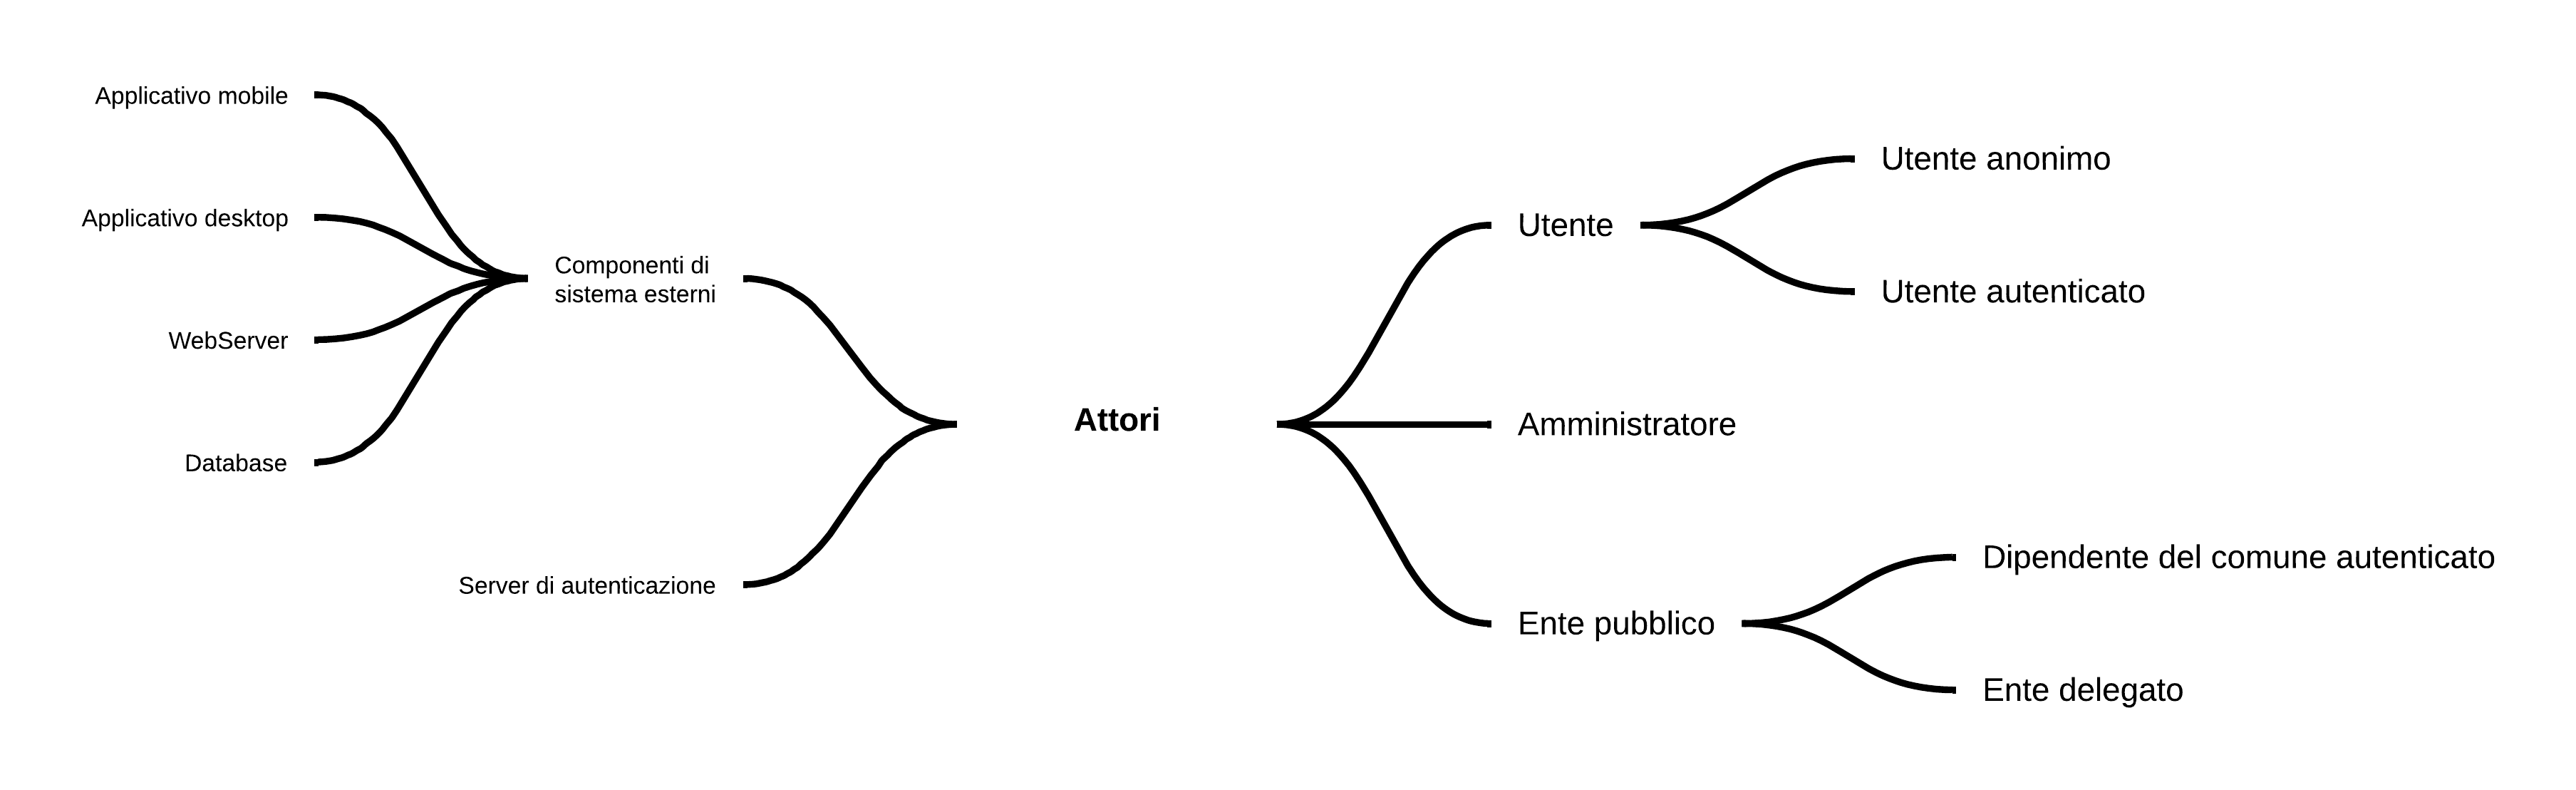
\includegraphics[width=1\textwidth]{Images/MindMap.png}
    \caption{Mind map degli attori che interagiscono con il sistema}
\end{figure}

Tramite la mind map è possibile avere una rappresentazione chiara degli attori che interagiscono con il sistema.\\
\clearpage

\section{Prototipo del sistema}
\index{Prototipo del sistema} % Aggiunge una voce all'indice

\subsection{Mockup applicazione mobile}
\index{Mockup applicazione mobile} % Aggiunge una voce all'indice\usepackage{makecell}

\subsubsection{Schermata principale}
\index{Schermata principale} % Aggiunge una voce all'indice
\begin{figure}[htbp]
    \label{4.1.1}
    \centering
    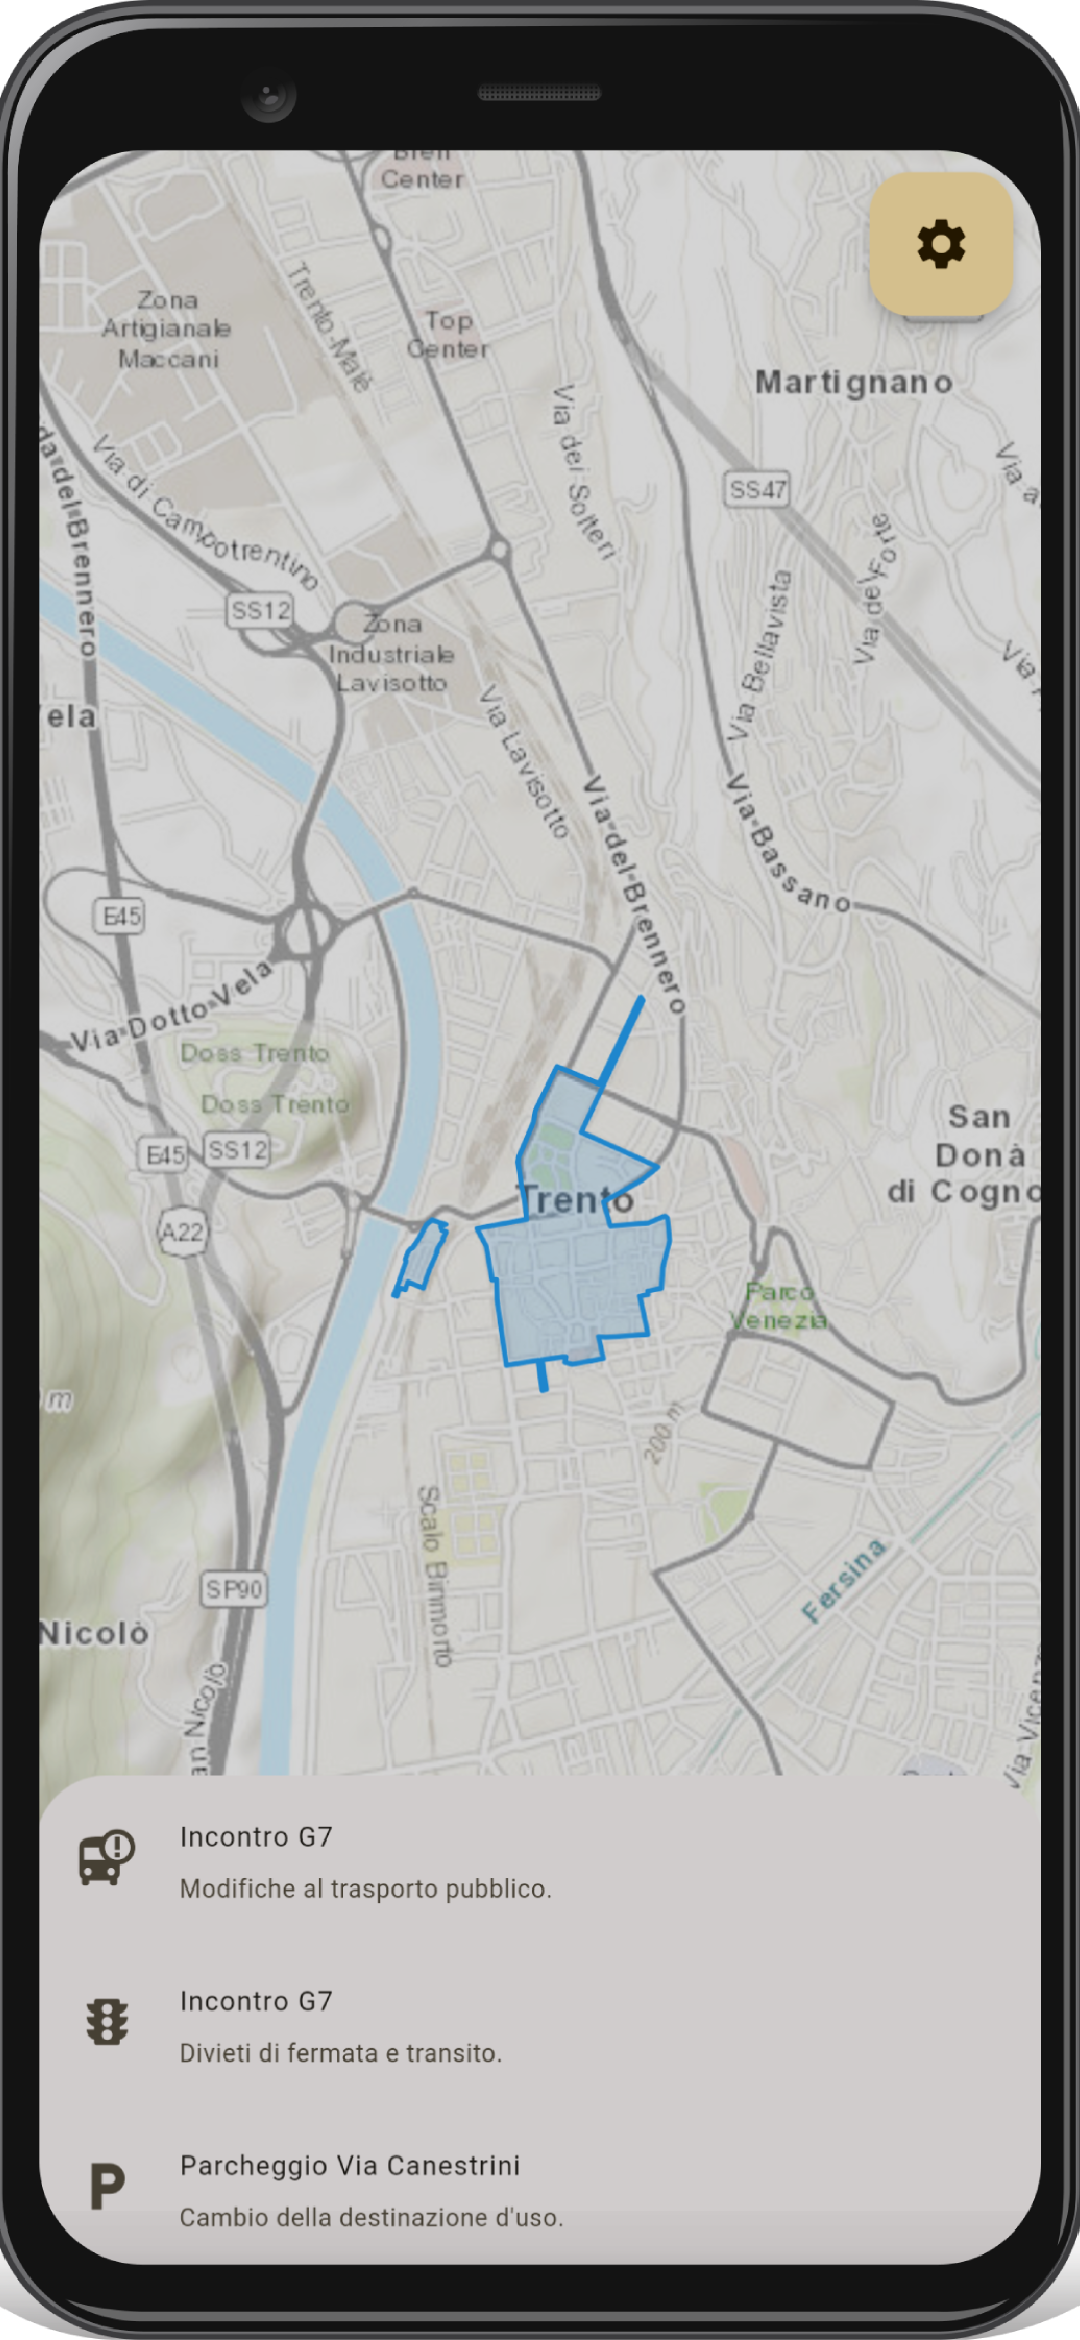
\includegraphics[width=0.35\textwidth]{Images/Mockup1 - Mobile.png}
    \caption{Mockup schermata principale dell'applicazione mobile}
\end{figure}

È rappresentata la schermata principale dell'\textit{applicazione mobile} che il cittadino installerà sul proprio smartphone.\\
La schermata principale mostra una mappa della città di Trento con le zone interessate dalle variazioni della viabilità.\\
La lista sottostante la mappa riporta tutte le variazioni presenti nel sistema che si trovano nel periodo di visualizzazione, con la possibilità di selezionare una variazione per visualizzarne i dettagli.\\
\clearpage

\subsubsection{Dettagli variazione selezionata}
\index{Dettagli variazione selezionata} % Aggiunge una voce all'indice
\begin{figure}[htbp]
    \label{4.1.2}
    \centering
    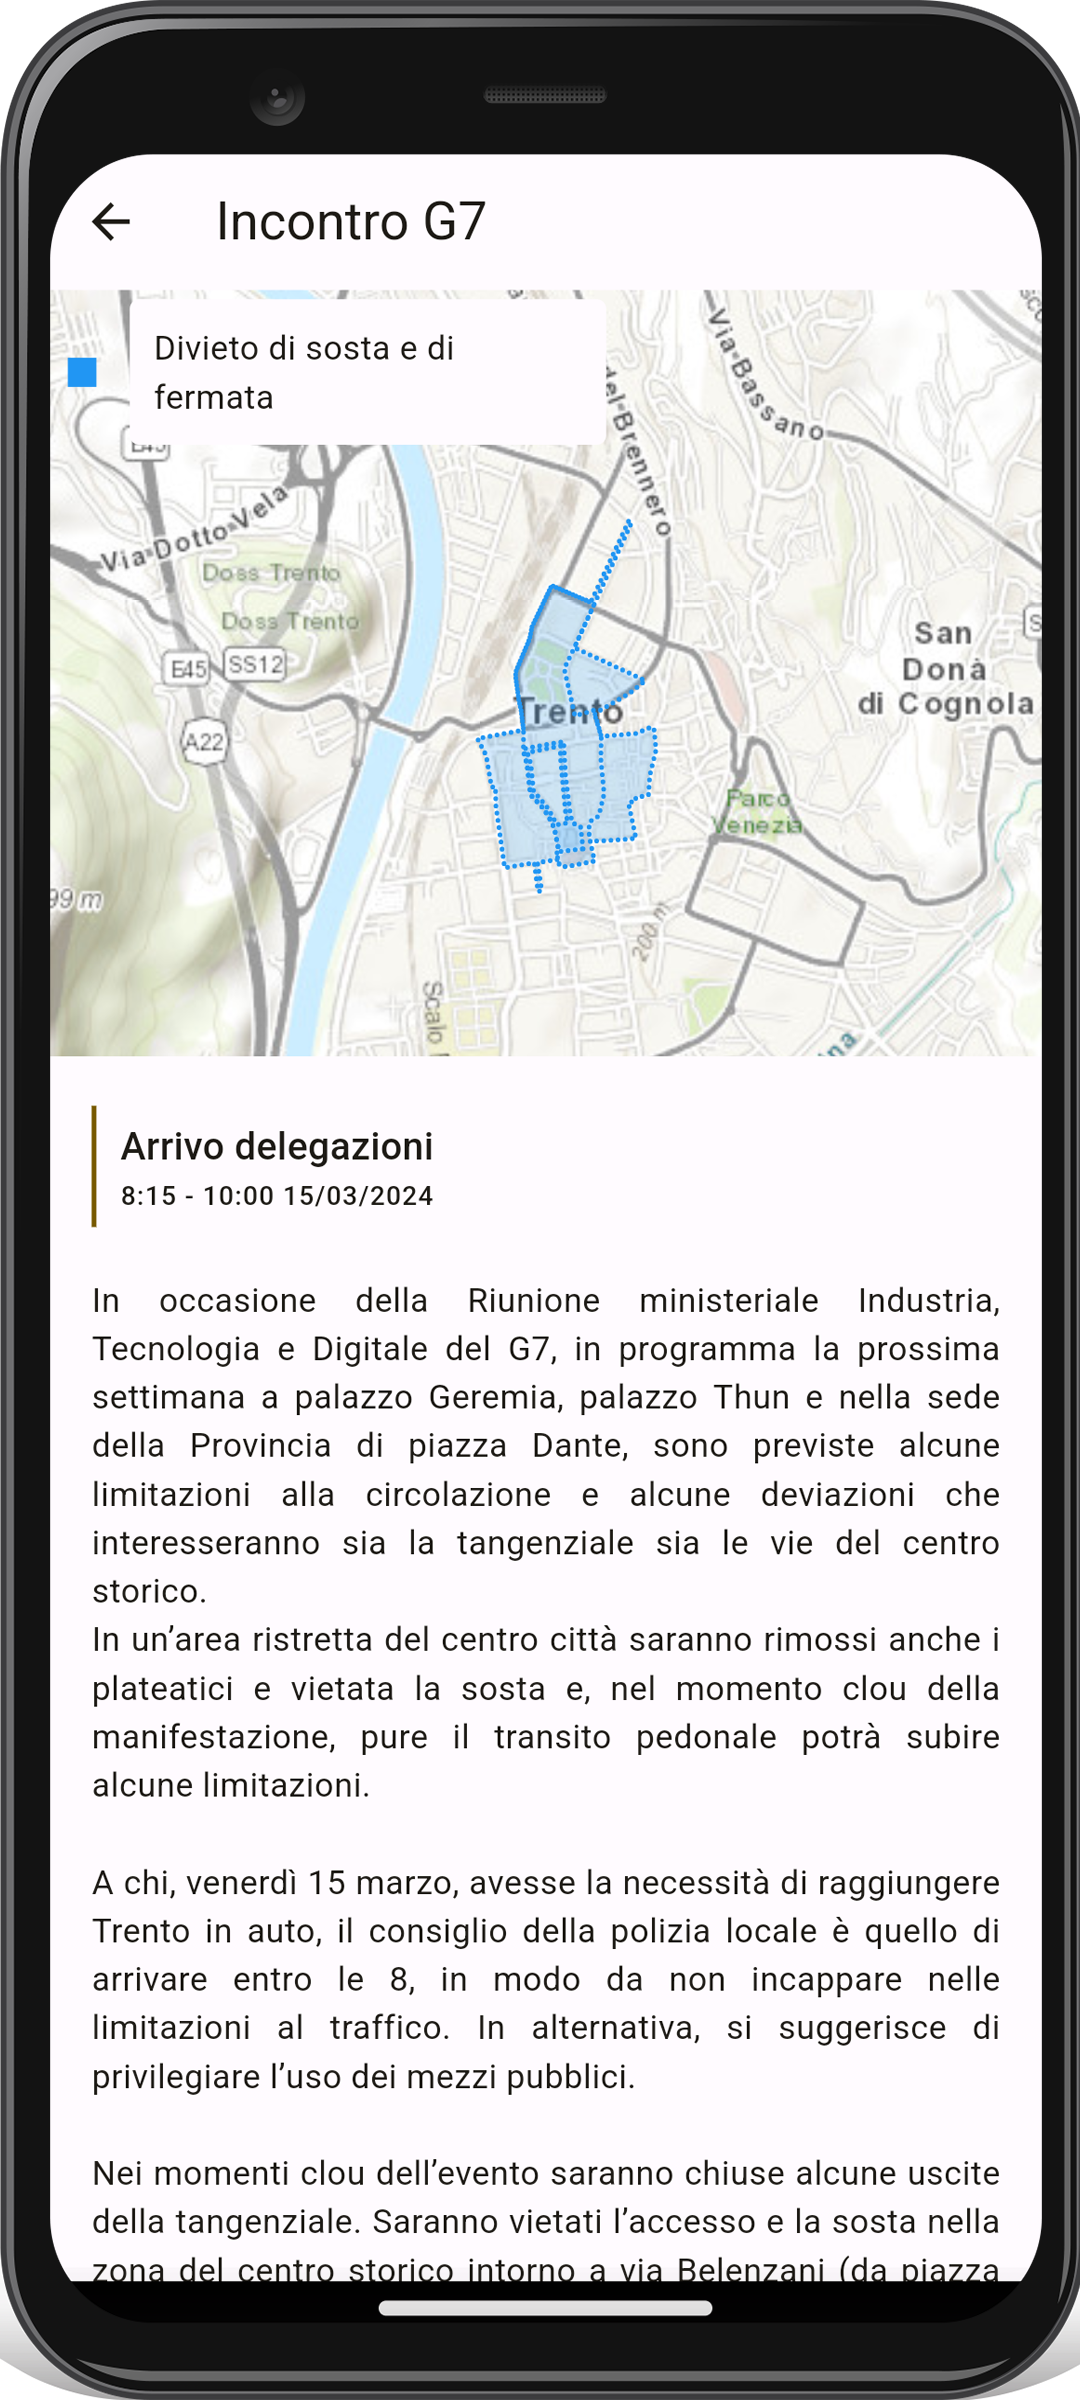
\includegraphics[width=0.35\textwidth]{Images/Mockup2 - Mobile.png}
    \caption{Mockup schermata detagli di un evento dell'applicazione mobile}
\end{figure}

In questo caso invece è riportata la schermata di visualizzazione dei dettagli di una variazione della viabilità.\\
È stato selezionato il precedente evento "Incontro G7", quindi sono visualizzati tutti i dettagli relativi a tale evento.\\
Nella fattispecie sono presenti la descrizione dell'evento, la data di inizio e fine, la zona interessata e la mappa con la visualizzazione della zona interessata.\\
Inoltre è presente un pulsante per tornare alla schermata principale dell'applicazione.\\
\clearpage

\subsubsection{Mockup notifiche degli eventi}
\index{Mockup notifiche degli eventi} % Aggiunge una voce all'indice

\begin{figure}[htbp]
    \label{4.1.3}
    \centering
    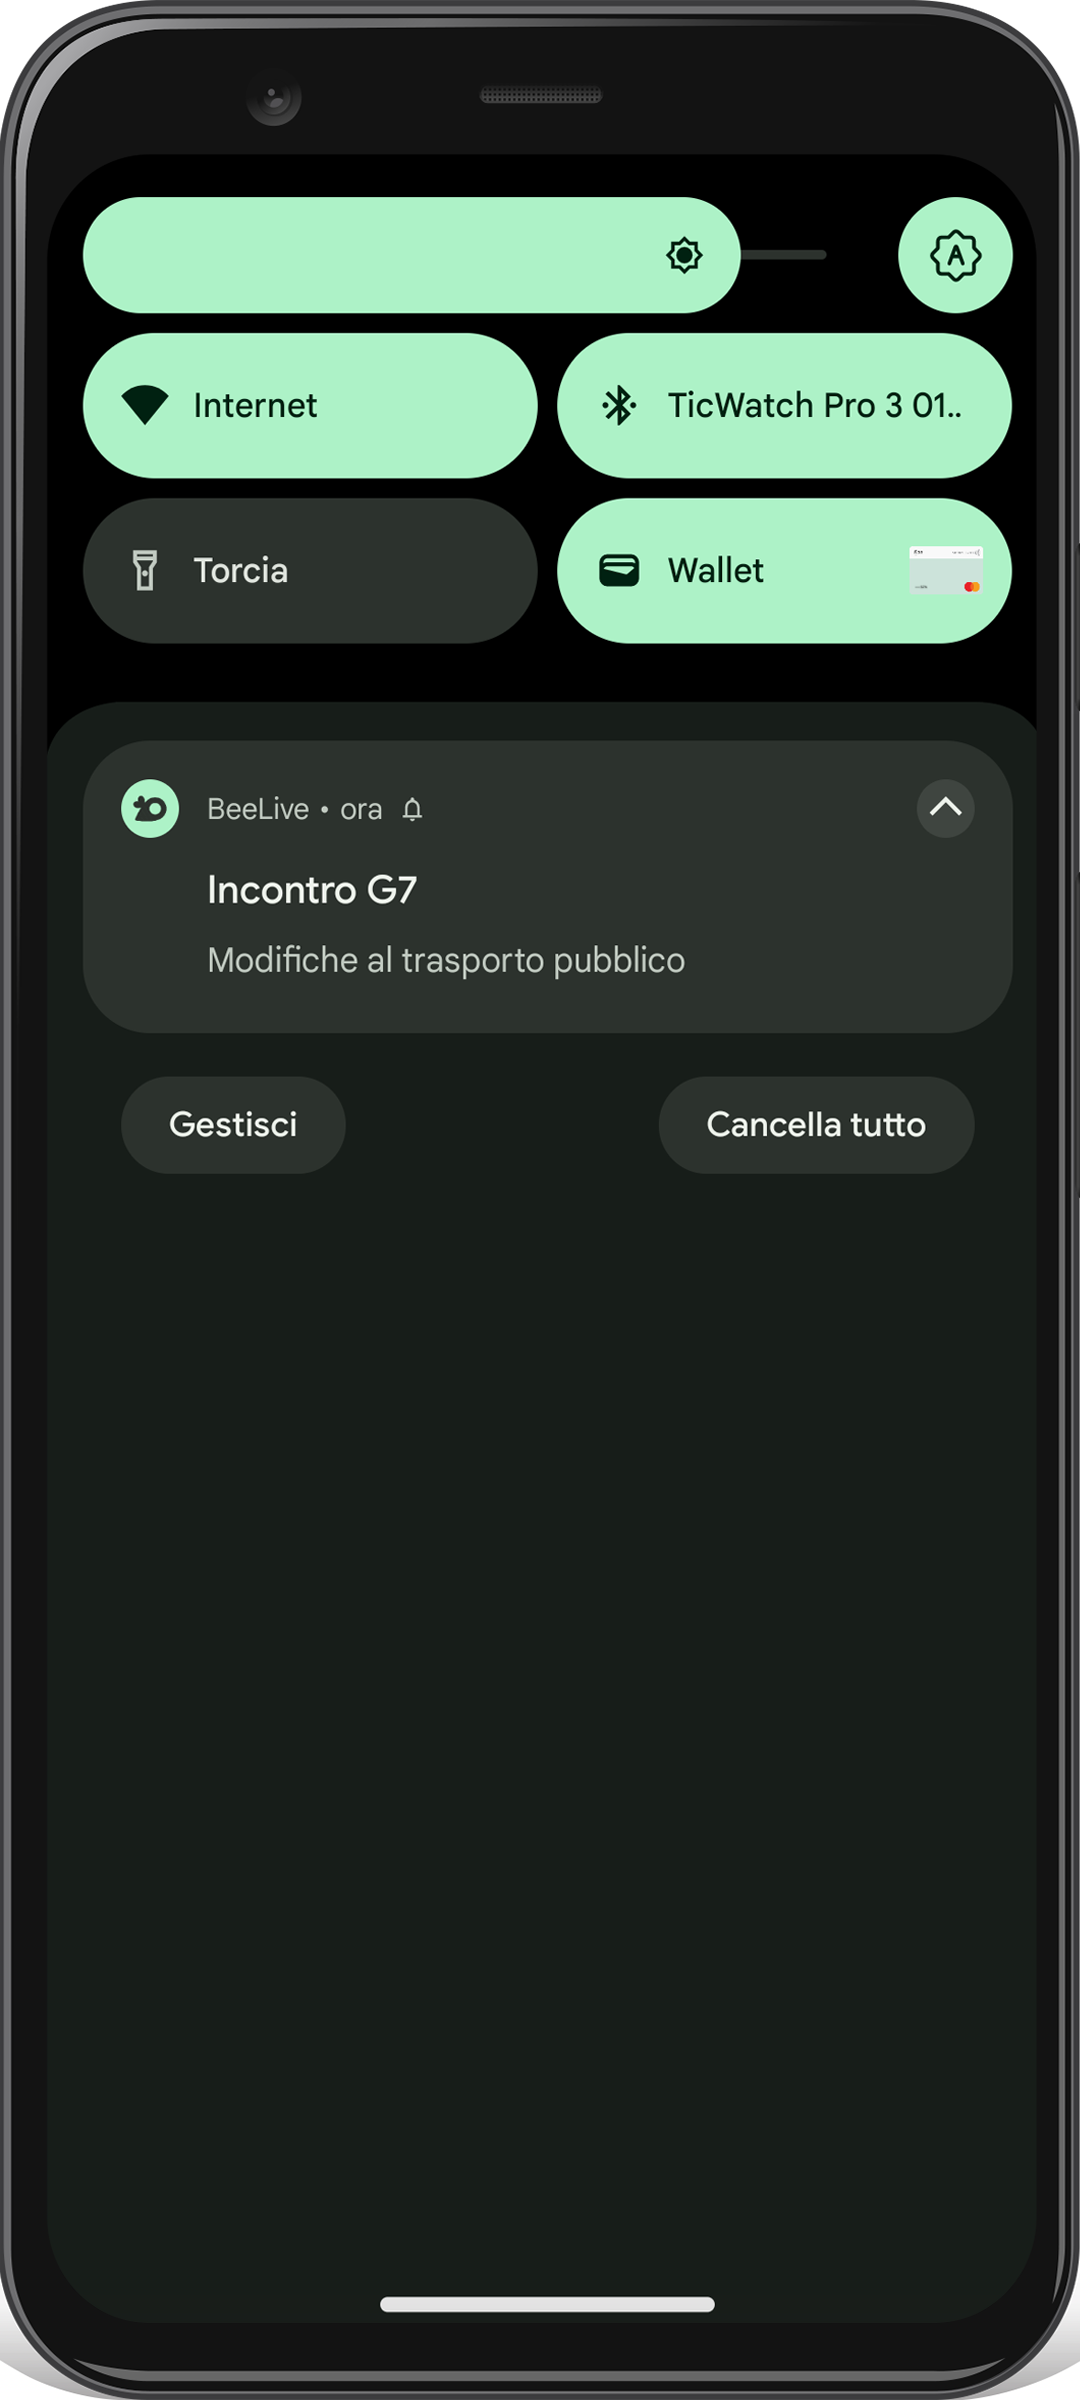
\includegraphics[width=0.35\textwidth]{Images/Mockup3 - Mobile.png}
    \caption{Mockup notifiche generate da un'evento dall'applicazione mobile}
\end{figure}

L'evento preso nell'esempio precedente era impostato per generare delle notifiche push.\\
Quella riportata nell'esempio soprastante rappresenta la notifica di inizio dell'evento "Incontro G7".\\
Interagendo con essa sarà quindi aperta l'applicazione mobile sulla schermata riportata in \hyperref[fig:Dettaglio_evento]{figura 2}, permettendo quindi la consultazione delle modifiche per intero.\\

\clearpage

\subsection{Mockup interfaccia desktop}
\index{Mockup interfaccia desktop} % Aggiunge una voce all'indice
%Immagine singola
\begin{figure}[htbp]
    \label{4.2}
    \centering
    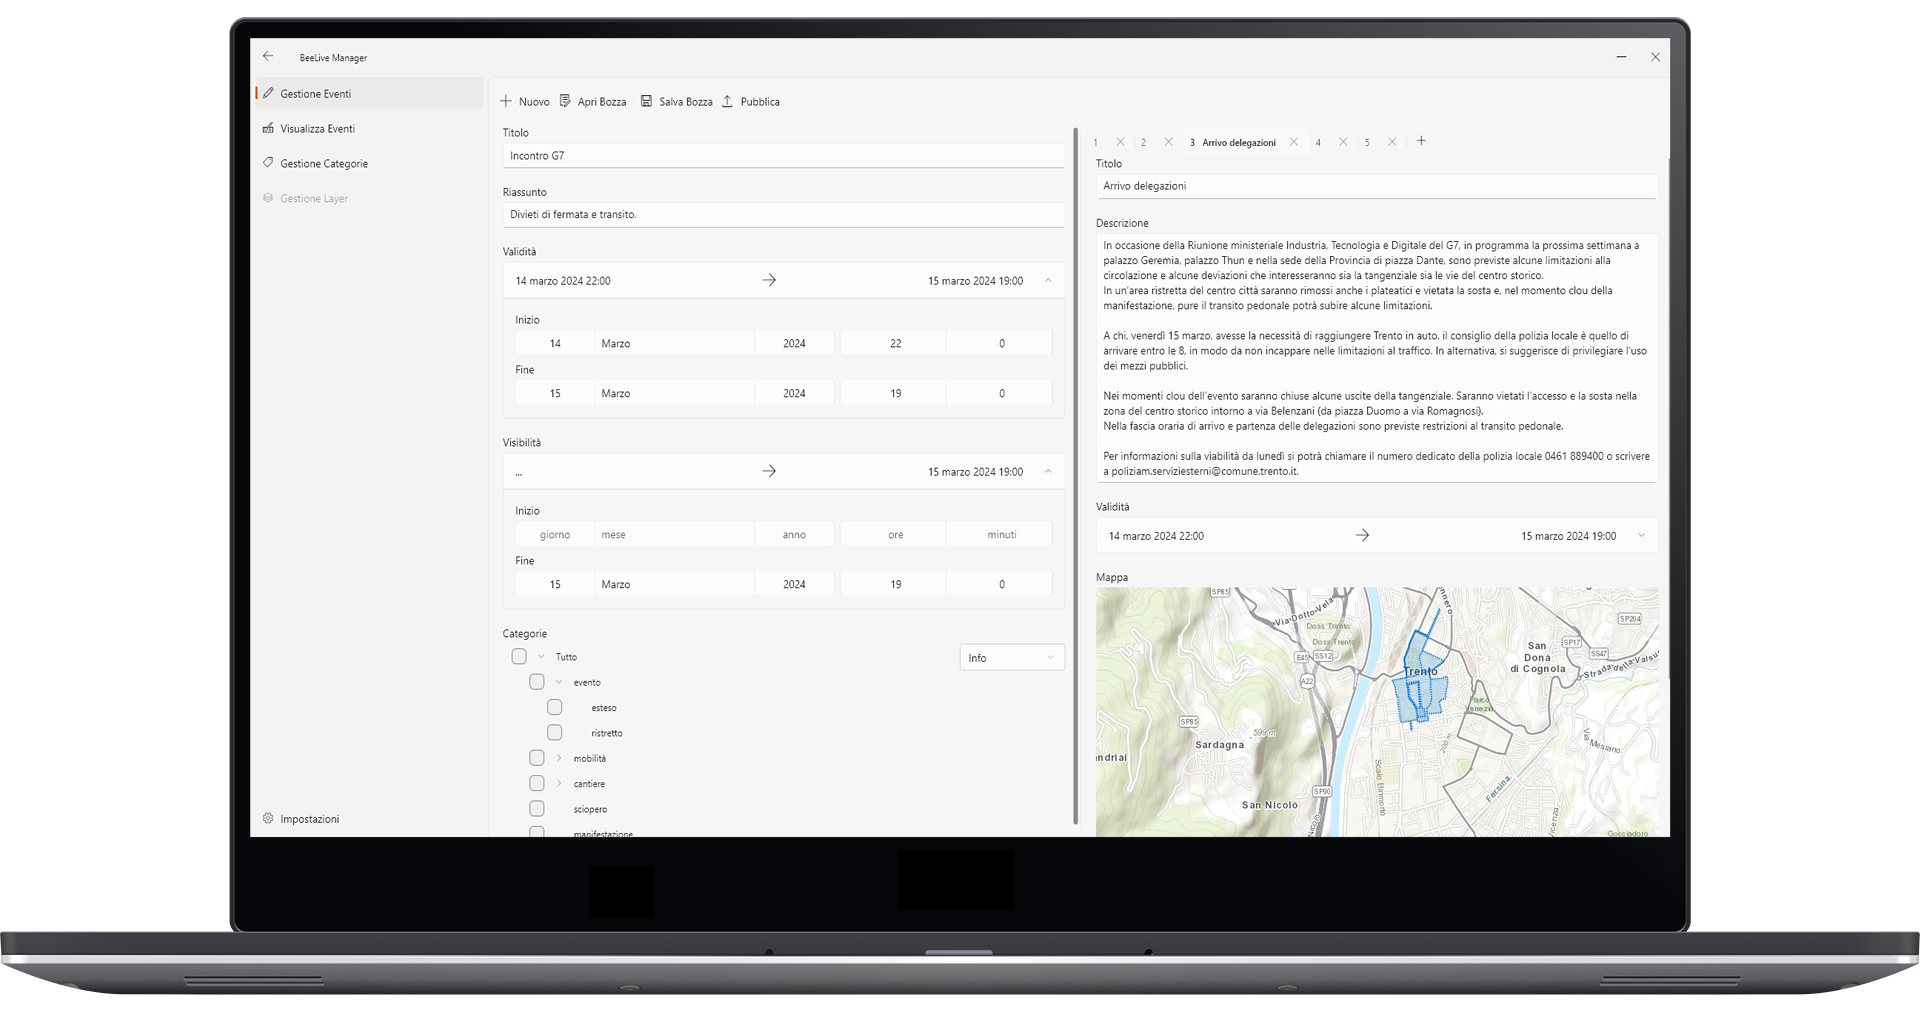
\includegraphics[width=1\textwidth]{Images/Mockup1 - Desktop.png}
    \caption{Mockup dell'interfaccia amministrativa}
\end{figure}

L'immagine rappresenta come dovrebbe essere strutturata l'interfaccia dell'\textit{applicativo desktop}, utilizzato dagli enti pubblici con potere di amministrazione per la pobblicazione degli eventi in città che ne influenzano la viabilità.\\
L'interfaccia comprende un menu laterale per la navigazione tra le varie sezioni dell'applicativo e la schermata dove il sottomenù selezionato presenta tutte le sue specifiche funzionalità disponibili.

Il sottomenù selezionato in questo caso è "Gestione Eventi", la sezione in cui è possibile inserire un nuovo evento che modifica la viabilità cittadina. Infatti sono riportati tutti i campi necessari per la creazione di un evento, come il titolo, il riassunto, la data di inizio e fine di validità dell'evento e di visibilità sull'applicativo mobile, e le categorie che caratterizzano l'evento.

L'interfaccia è strutturata in modo che ogni evento abbia la possibilità di essere composto da più sottoeventi. Nella sezione di destra è possibile visualizzare l'inderimento del sottoevento "Arrivo delle delegazioni", dove è possibile inserire il titolo, la descrizione, la data di validità e la zona interessata direttamente su mappa.\\

\clearpage

\section{Requisiti Funzionali}
\index{Requisiti funzionali}

\subsection{Utente anonimo tramite applicativo mobile}
\index{Utente anonimo tramite applicativo mobile} % Aggiunge una voce all'indice

\subsubsection{Deve poter visualizzare la lista degli eventi (core)}\label{Requirements:Lista}
\index{Deve poter visualizzare la lista degli eventi} % Aggiunge una voce all'indice
\label{5.1.1}
L'utente anche se non autenticato a sistema deve avere la possibilità di visualizzare la lista intera di tutti gli eventi pubblicati.

\subsubsection{Deve poter filtrare gli eventi per categoria}
\index{Deve poter filtrare gli eventi per categoria} % Aggiunge una voce all'indice
\label{5.1.2}
Gli eventi sono divisi in categorie, l'utente deve avere la possibilità di esprimere le proprie preferenze sugli eventi da visualizzare in lista definita in \ref{Requirements:Lista}.

\subsubsection{Deve poter nascondere eventi specifici che non gli interessano}
\index{Deve poter nascondere eventi specifici che non gli interessano} % Aggiunge una voce all'indice
\label{5.1.3}
In caso l'utente non dimostri interesse per un evento specifico, deve avere la possibilità di nasconderlo dalla lista degli eventi.

\subsubsection{Deve poter visualizzare gli eventi su mappa (core)}
\index{Deve poter visualizzare gli eventi su mappa} % Aggiunge una voce all'indice
\label{5.1.4}
L'utente deve essere in grado di visualizzare in modo intuitivo l'area fisica interessata dagli eventi di suo interesse. 

\subsubsection{Deve potersi registrare senza perdita di impostazioni}
\index{Deve potersi registrare senza perdita di impostazioni} % Aggiunge una voce all'indice
\label{5.1.5}
Le impostazioni selezionate da un utente anonimo non devono essere perse nel caso in cui questo si registri a sistema.

\subsubsection{Deve potersi autenticare}
\index{Deve potersi autenticare} % Aggiunge una voce all'indice
\label{5.1.6}
Gli utenti devono avere la possibilità di autenticarsi a sistema per usufruire della sincronizzazione tra dispositivi.

\subsubsection{Deve poter indicare categorie di interesse}
\index{Deve poter indicare categorie di interesse} % Aggiunge una voce all'indice
\label{5.1.7}
Deve poter indicare categorie di interesse in maniera indipendente per eventi in \textit{zone di interesse} (Aree e percorsi) e non.
\begin{itemize}
    \item Granularità maggiori (ad esempio: per zona di interesse e per label di rischio) non sono previste, in quanto rischiano di compromettere l'user experience
\end{itemize}

\subsubsection{Deve poter indicare aree di interesse}
\index{Deve poter indicare aree di interesse} % Aggiunge una voce all'indice
\label{5.1.8}
L'utente deve poter indicare delle zone su mappa per cui dimostra più interesse.

\subsubsection{Deve poter indicare percorsi di interesse}
\index{Deve poter indicare percorsi di interesse} % Aggiunge una voce all'indice
\label{5.1.9}
L'utente deve poter indicare dei percorsi su mappa per cui dimostra più interesse.

\subsubsection{Deve poter ricevere notifiche riguardo agli eventi}
\index{Deve poter ricevere notifiche riguardo agli eventi} % Aggiunge una voce all'indice
\label{5.1.10}
L'utente deve poter essere notificato all'insorgere di determinati eventi, sopratutto se tali eventi incorrono in un area o un percorso d'interesse indicato dall'utente

\subsection{Utente autenticato tramite applicativo mobile}
\index{Utente autenticato tramite applicativo mobile} % Aggiunge una voce all'indice

\subsubsection{Deve avere le impostazioni sincronizzate tra i vari dispositivi}
\index{Deve avere le impostazioni sincronizzate tra i vari dispositivi} % Aggiunge una voce all'indice
\label{5.2.1}
Siccome l'utente autenticato tramite applicativo mobile eredita le caratteristiche dell'utente anonimo, valgono tutti i suoi requisiti, con l'aggiunta che in questo caso l'utente ha tutte le impostazioni sincronizzate tra tutti i dispositivi in cui è autenticato.

\subsection{Dipendente autorizzato del Comune di Trento tramite applicativo desktop}
\index{Dipendente autorizzato del Comune di Trento tramite applicativo desktop} % Aggiunge una voce all'indice

\subsubsection{Deve poter definire sottocategorie}
\index{Deve poter definire sottocategorie}
\label{5.3.1}
Il dipendente deve poter definire delle categorie e sottocategorie (organizzate in modo gerarchico in modo da migliorare la granularità del filtraggio degli eventi) alle quali un evento appartiene. 

\subsubsection{Deve poter gestire gli eventi di sua competenza (core)}
\index{Deve poter gestire gli eventi di sua competenza}
\label{5.3.2}
La gestione degli eventi di un dipendente include la creazione, la modifica, l'eliminazione e la pubblicazione (solo se \textit{trusted}) degli eventi di sua competenza.

\subsubsection{Non deve poter gestire gli eventi che non sono di sua competenza}
\index{Non deve poter gestire gli eventi che non sono di sua competenza}
\label{5.3.3}
Il dipendente ha accesso solamente alle operazioni riguardanti gli eventi di sua competenza e non può gestire tutti gli altri.

\subsubsection{Deve poter risalire al dipendente autorizzato che ha gestito un evento specifico}
\index{Deve poter risalire al dipendente autorizzato che ha gestito un evento specifico}
\label{5.3.4}
Deve sempre essere possibile inividuare gli utenti autorizzati dal comune che hanno eseguito azioni sugli eventi pubblicati a sistema.

\subsubsection{Deve poter visionare lo storico della gestione degli eventi}
\index{Deve poter visionare lo storico della gestione degli eventi}
\label{5.3.5}
L'utente autorizzato deve poter visionare lo storico delle interazioni sugli eventi, con la possibilità di visionare chi ha effettuato l'attività e quando.

\subsubsection{Deve poter definire elementi geografici di interesse per facilitare la selezione delle aree interessate all'evento}
\index{Deve poter definire elementi geografici di interesse per facilitare la selezione delle aree interessate all'evento}
\label{5.3.6}
Per facilitare la selezione delle aree interessate all'evento, l'utente autorizzato deve poter definire elementi geografici notevoli.

\subsubsection{Deve poter sospendere la gestione di un evento e riprenderla successivamente}
\index{Deve poter sospendere la gestione di un evento e riprenderla successivamente}
\label{5.3.7}
Si deve avere la possibilità di sospendere la gestione di un evento, potendola riprendere successivamente senza alcuna perdita di dati.

\subsubsection{Deve poter caricare elementi geografici provenienti da file esterni}
\index{Deve poter caricare elementi geografici provenienti da file esterni}
\label{5.3.8}
L'utente, in fase di pubblicazione di un nuovo evento, deve avere la possibilità di indicare la zona d'interesse tramite il caricamento di un file contenente tutte le sue informazioni geografiche.

\subsubsection{Deve poter creare un evento a partire da file di strutture specifiche}
\index{Deve poter creare un evento a partire da file con strutture specifiche}
\label{5.3.9}
I dipartimenti devono poter continuare ad utilizzare i loro file attuali che determinano e caratterizzano gli eventi per la loro gestione sul sistema.

\subsubsection{Deve avere esclusività di gestione durante il corso dell'operazione}
\index{Deve avere esclusività di gestione durante il corso dell'operazione}
\label{5.3.10}
Durante l'operazione di gestione di un evento, l'utente deve avere l'esclusività di gestione, impedendo ad altri utenti di effettuare modifiche.

\subsection{Enti delegati tramite API gestionali del Web Server}
\index{Enti delegati tramite API gestionali del Web Server}
Questo attore eredita le capacità di "Dipendente autorizzato del Comune di Trento", integrandone le caratteristiche.

\subsection{Amministratore di sistema}
\index{Amministrazione di sistema}
\label{5.4.1}

\subsubsection{Deve poter gestire le policies di access control}
\index{Deve poter gestire le policies di access control}
\label{5.5.1}
Essendo l'amministratore di sistema, ha il compito di gestire tutte le policies di access control del sistema.

\subsubsection{Deve poter definire le aree di competenza delle entità di gestione}
\index{Deve poter definire le aree di competenza delle entità di gestione}
\label{5.5.2}
È compito suo definire tutte le aree di competenza di \textit{Dipendenti autorizzati del Comune di Trento} e \textit{Enti delegati}.

\subsubsection{Deve avere accesso privilegiato al sistema}
\index{Deve avere accesso privilegiato al sistema}
\label{5.5.3}
Deve avere libertà nell'apportare modifiche specifiche alle componenti (come il salvataggio dei dati)

\subsubsection{Deve poter definire le entità di gestione come \textit{trusted} o \textit{un-trusted}}
\index{Deve poter definire le entità di gestione come \textit{trusted} o \textit{un-trusted}}
\label{5.5.4}
È necessaria questa distinzione, solamente gli utenti \textit{trusted} possono accedere ai servizi offerti dal sistema.

\subsection{WebServer}
\index{WebServer}

\subsubsection{Deve garantire l'accesso al servizio ai soli utenti autorizzati}
\index{Deve garantire l'accesso al servizio ai soli utenti autorizzati}
\label{5.6.1}
Solamente gli utenti autorizzati (Anche i non autenticati, solo per alcuni servizi) possono accedere al servizio.

\subsection{DataBase}
\index{DataBase}

\subsubsection{Deve poter eseguire query spaziali}
\index{Deve poter eseguire query spaziali}
\label{5.7.1}
Sul DataBase sono salvati anche dati caratterizzati da coordinate. Deve essere possibile eseguire operazioni di ricerca su di esse.

\clearpage

\section{Requisiti non funzionali}
\index{Requisiti non funzionali} % Aggiunge una voce all'indice

\subsubsection{L'utente autenticato non deve avere altri vantaggi rispetto all'utente non autenticato}
\index{L'utente autenticato non deve avere altri vantaggi rispetto l'utente non autenticato} % Aggiunge una voce all'indice
L'applicativo deve poter essere utilizzato in maniera completa senza forzare l'autenticazione dell'utente, che ne comporta una barriera d'utilizzo, salvo eventuali problematiche implementative.

\subsubsection{Affidabilità dei dati forniti}
\index{Affidabilità dei dati forniti}
Tutti i dati che provengono dagli enti delegati devono essere considerati affidabili dal resto del sistema.

\subsubsection{Usabilità}
\index{Usabilità} % Aggiunge una voce all'indice
Per quanto riguarda l'\textit{applicazione mobile}, i cittadini devono essere in grado di utilizzarla dal primo momento in cui è intallata sul dispositivo.\\
Per invece l'\textit{applicativo desktop}, precedentemente al primo utilizzo è necessaria al più una specificazione delle funzionalità per il loro completo utilizzo.

\subsubsection{Scalabilità}
\index{Scalabilità} % Aggiunge una voce all'indice
Il requirement di scalabilità riguarda solamente l'\textit{applicazione mobile}, perchè deve essere in grado di gestire un elevato numero di utenti, che rispecchi il numero dgli abitanti di Trento.\\
L'\textit{applicativo desktop} invece non ha bisogno di scalabilità, in quanto è utilizzato solo da un numero limitato di utenti.

\subsubsection{Robustness}
\index{Robustness} % Aggiunge una voce all'indice
Un guasto al webserver di visualizzazione non deve compromettere il funzionamento del webserver di gestione, e viceversa.

\subsubsection{Prestazioni di notifica}
\index{Prestazioni di notifica} % Aggiunge una voce all'indice
La notifica di un nuovo evento deve raggiungere tutti i dispositivi mobili, connessi ad internet e con l'applicazione installata, entro un tempo di 10 minuti

\subsubsection{Reliability}
\index{Reliability} % Aggiunge una voce all'indice
Il sistema non deve essere soggetto a errori imprevisti di alcun tipo, ed eventuali bug non devono compromettere eventuali dati sensibili presenti sul server.\\
Il sistema gestionale usato dagli utenti autorizzati non deve essere soggetto a vulnerabilità che ne compromettano la sicurezza. 

\subsubsection{WebServer diviso}
\index{WebServer diviso}
Ci sono tre webserver: uno inerente il gestionale desktop, uno per gestire l'aplicazione mobile e uno dedicato alle notifiche.

\subsubsection{Tipologia di DataBase}
\index{Tipologia di DataBase}
Deve essere utilizzato il DataBase non relazionale MongoDB.

\clearpage

\section{Grafi BPMN}
\index{Grafi BPMN} % Aggiunge una voce all'indice

\subsection{Utente mobile}
\index{Utente mobile}

\subsubsection{Autenticazione}
\index{Autenticazione}

\begin{figure}[htbp]
    \label{7.1.1}
    \centering
    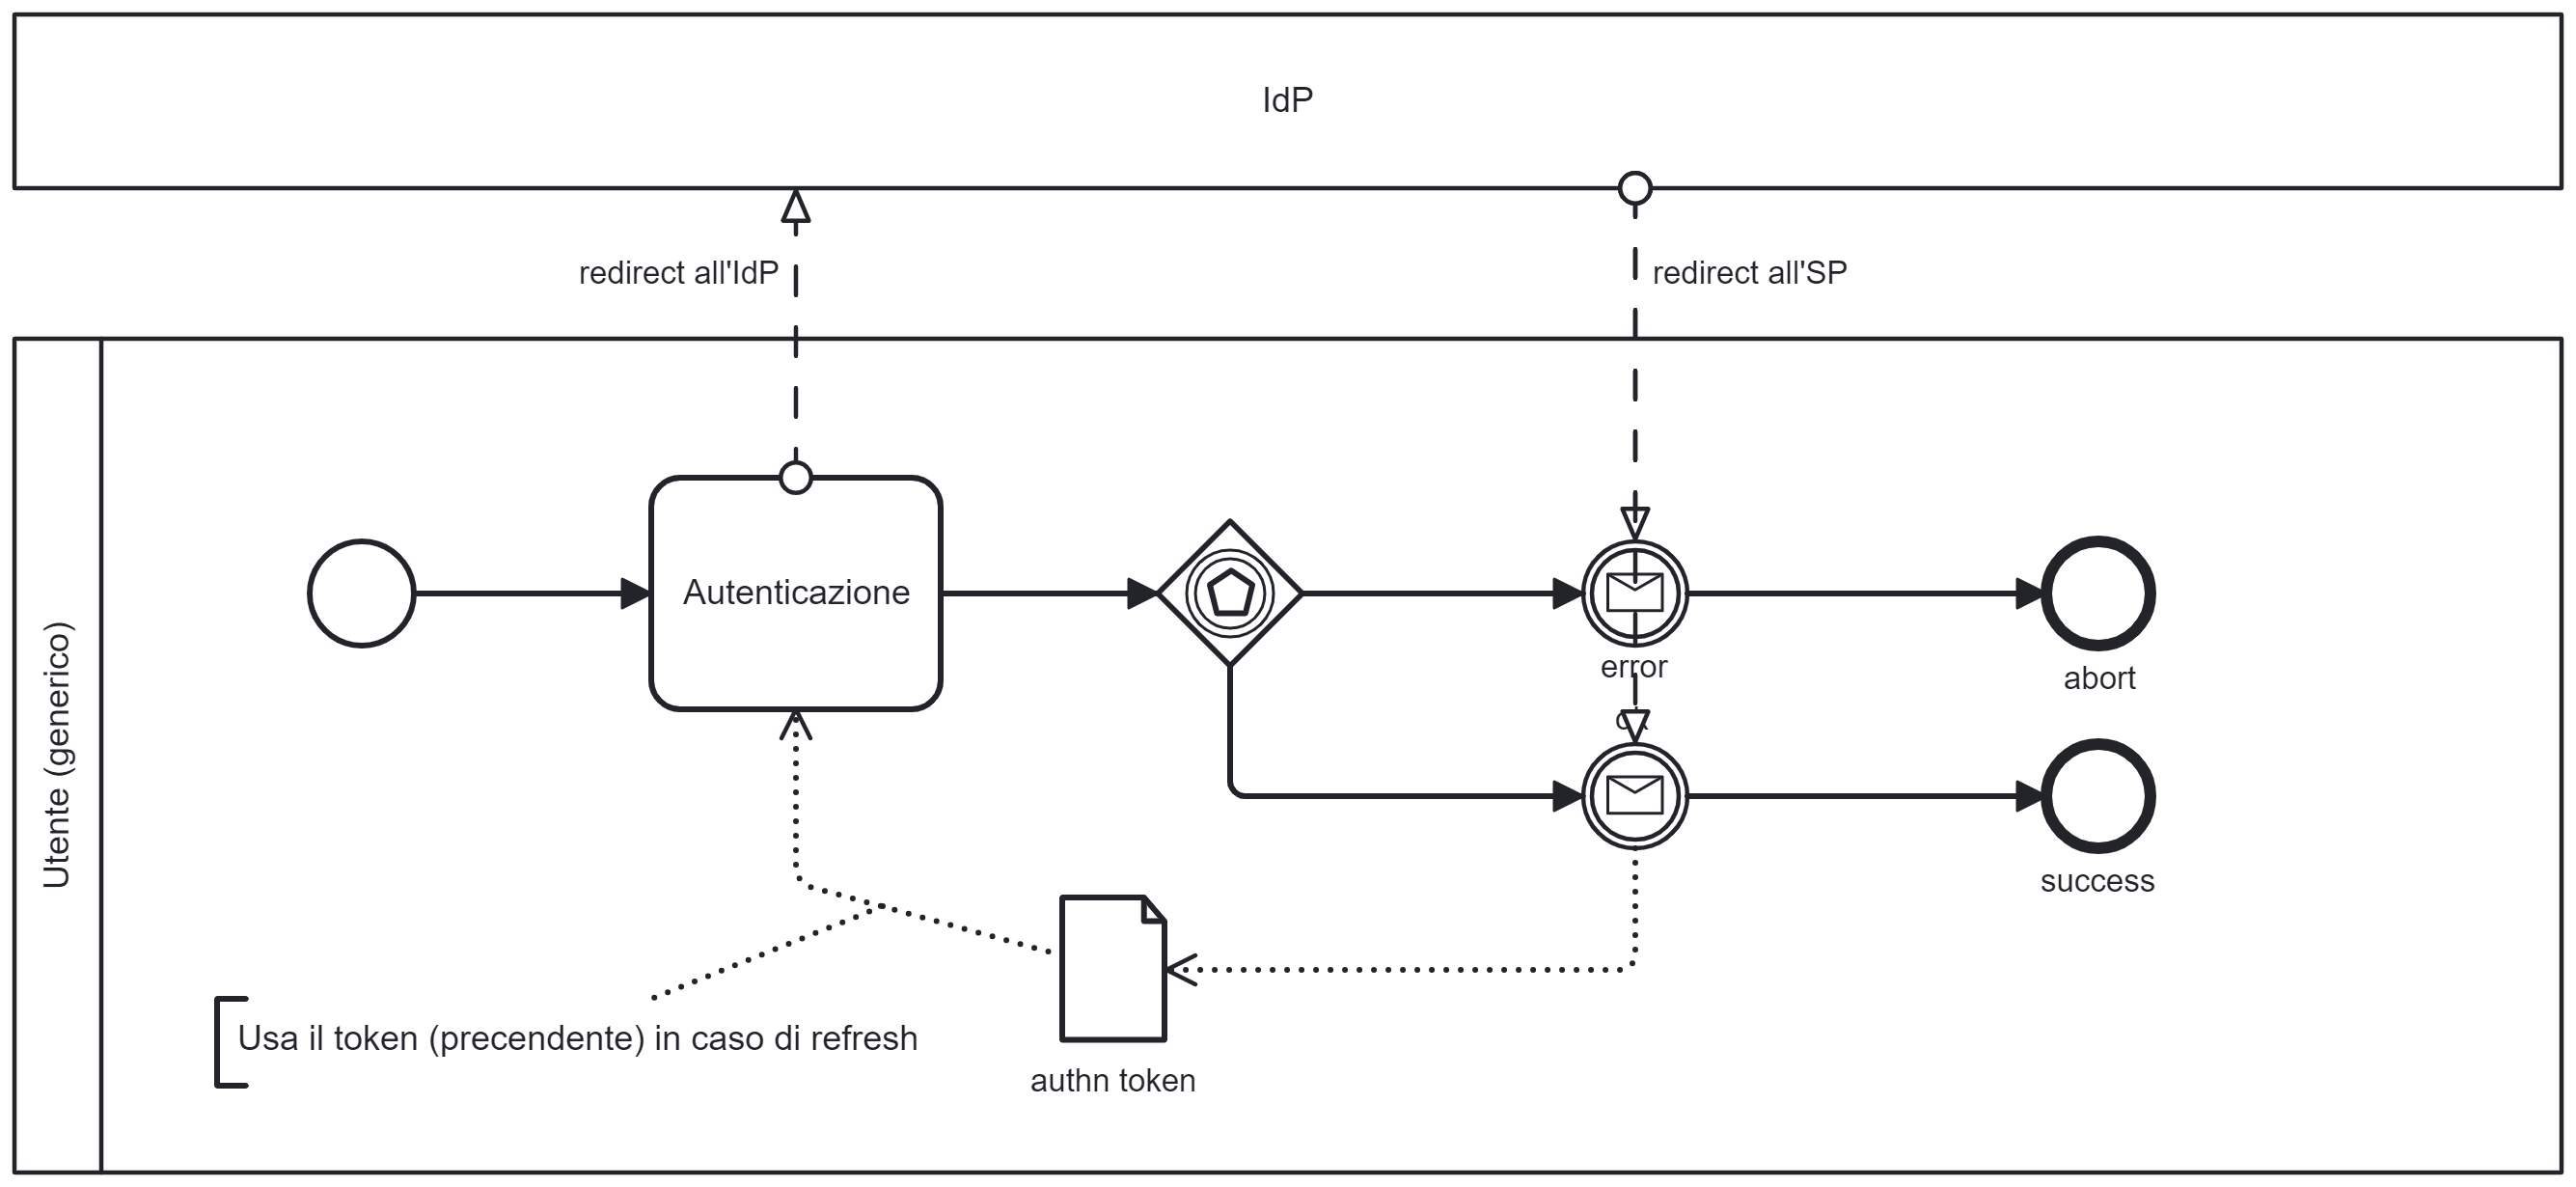
\includegraphics[width=1\textwidth]{Images/BPMN - authn.png}
    \caption{Grafo BPMN per l'autenticazione dell'utente}
\end{figure}

\clearpage

\subsubsection{Autorizzazione}
\index{Autorizzazione}

\begin{figure}[htbp]
    \label{7.1.2}
    \centering
    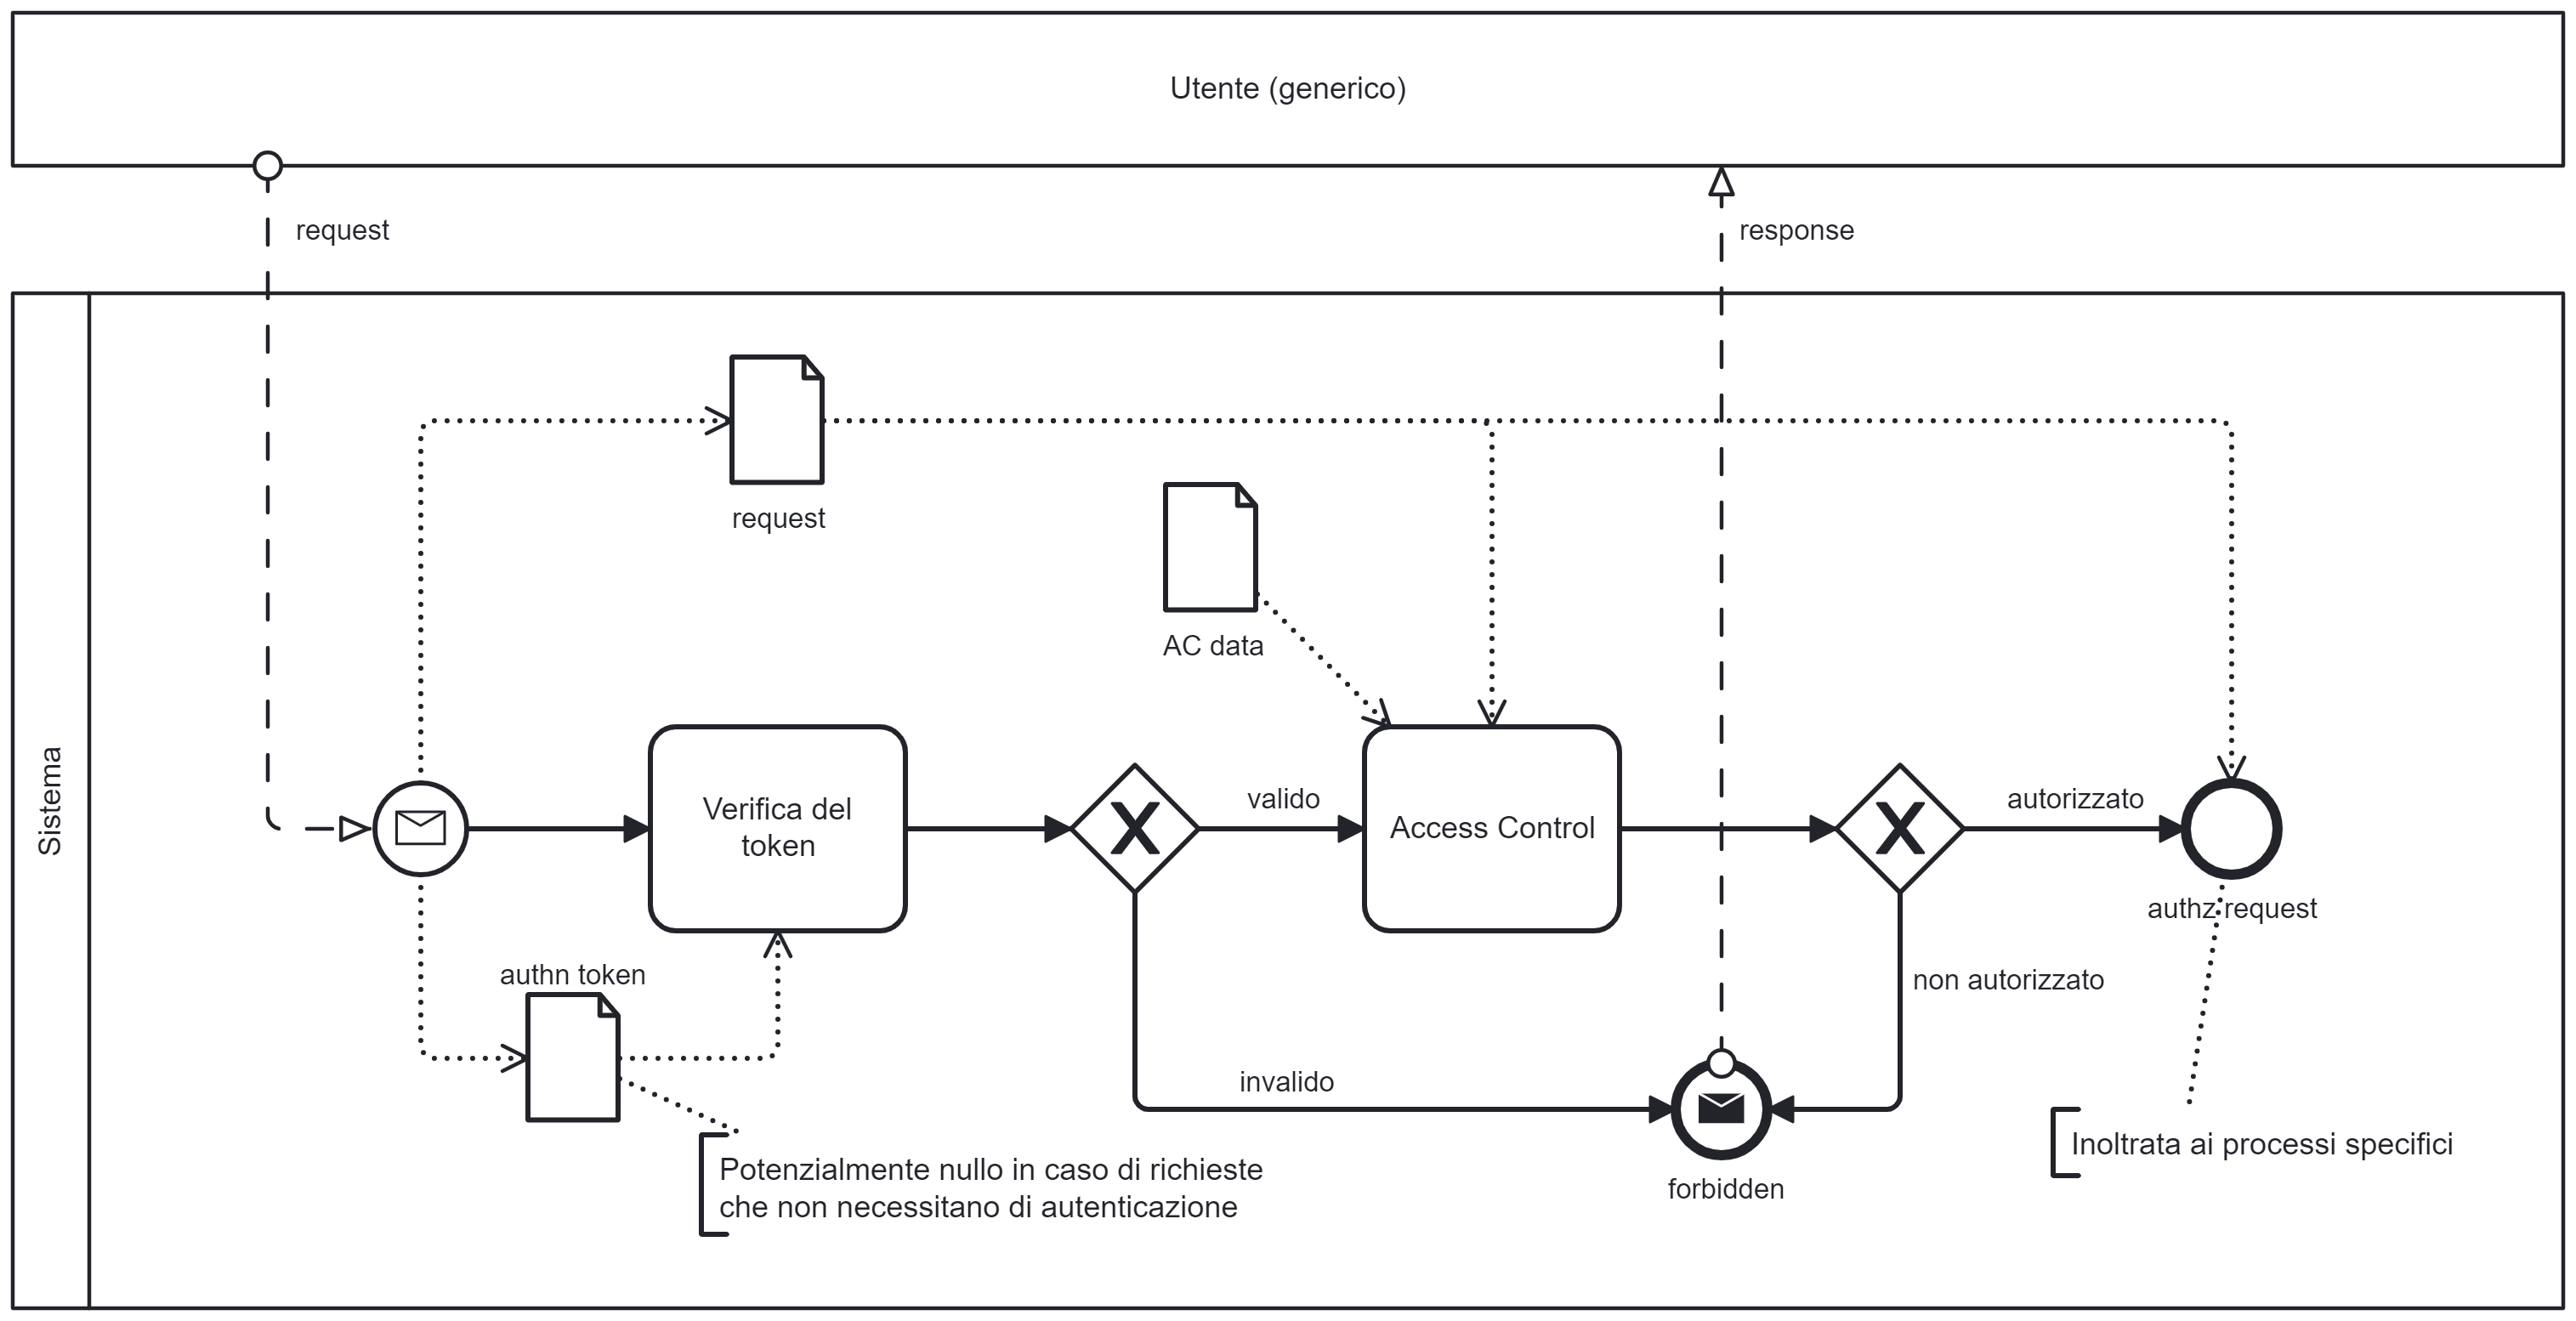
\includegraphics[width=1\textwidth]{Images/BPMN - authz.png}
    \caption{Grafo BPMN per l'autorizzazione dell'utente}
\end{figure}

\clearpage

\subsubsection{Lista degli eventi}
\index{Lista degli eventi}

\begin{figure}[htbp]
    \label{7.1.3}
    \centering
    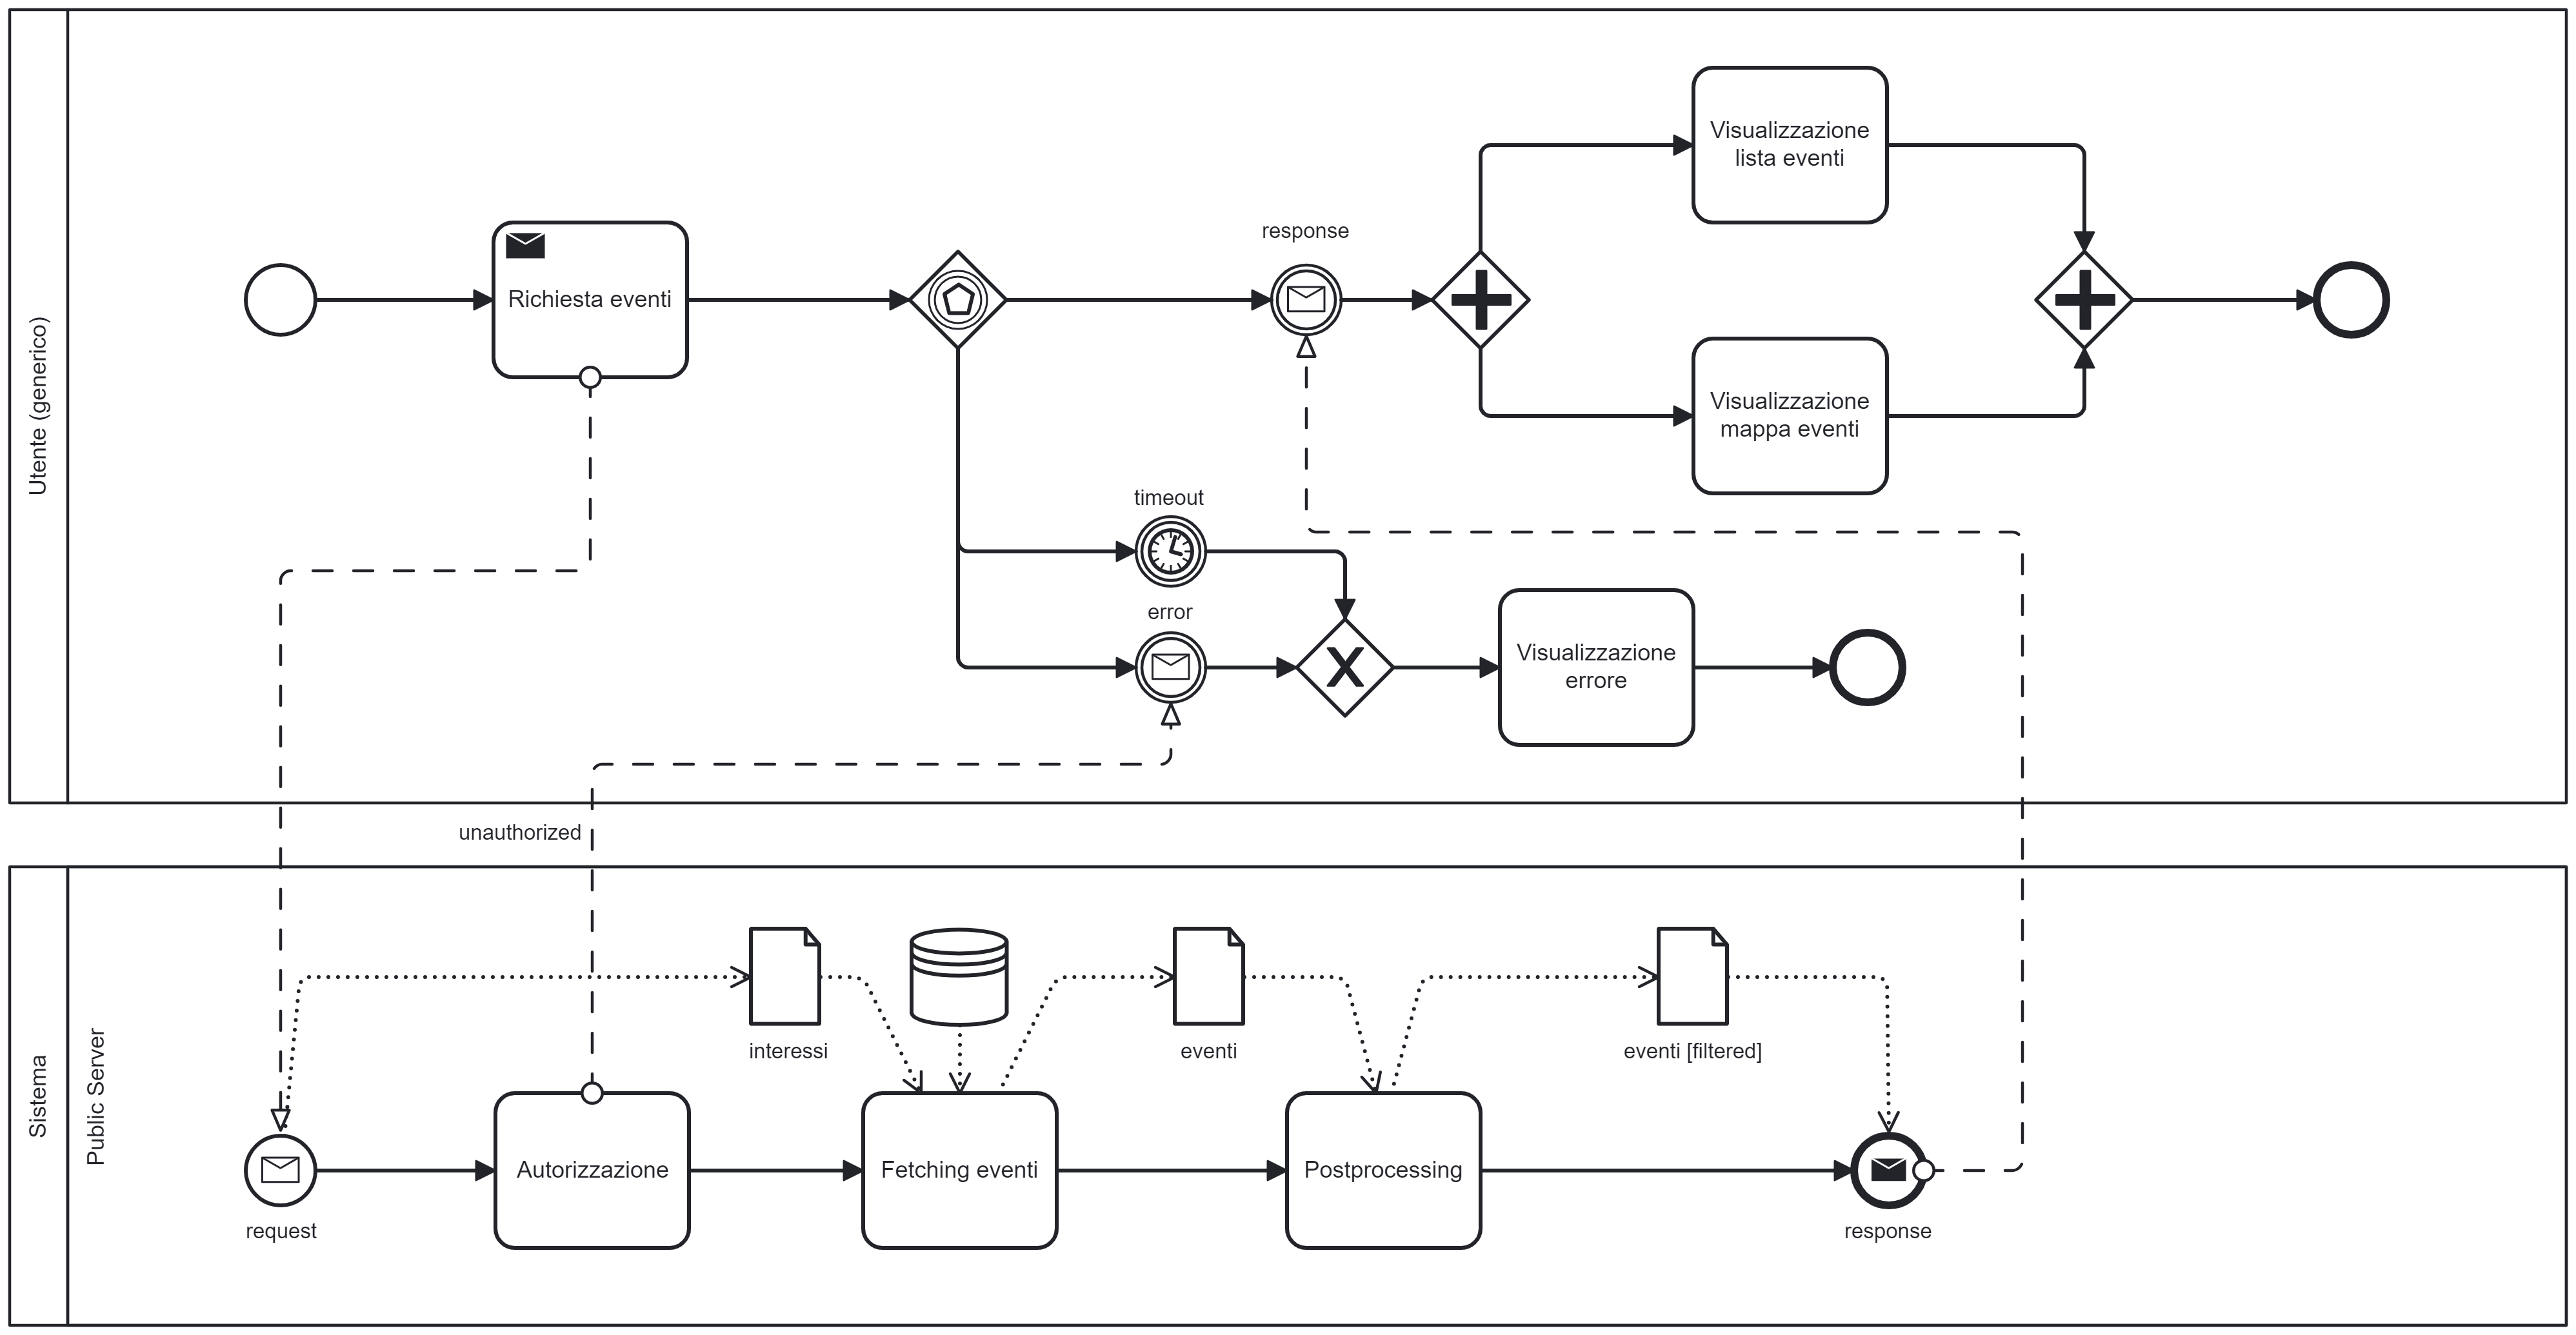
\includegraphics[width=1\textwidth]{Images/BPMN - list.png}
    \caption{Grafo BPMN per la visualizzazione della lista degli eventi}
\end{figure}

\clearpage

\subsubsection{Visualizzazione dettagli evento}
\index{Visualizzazione dettagli evento}

\begin{figure}[htbp]
    \label{7.1.4}
    \centering
    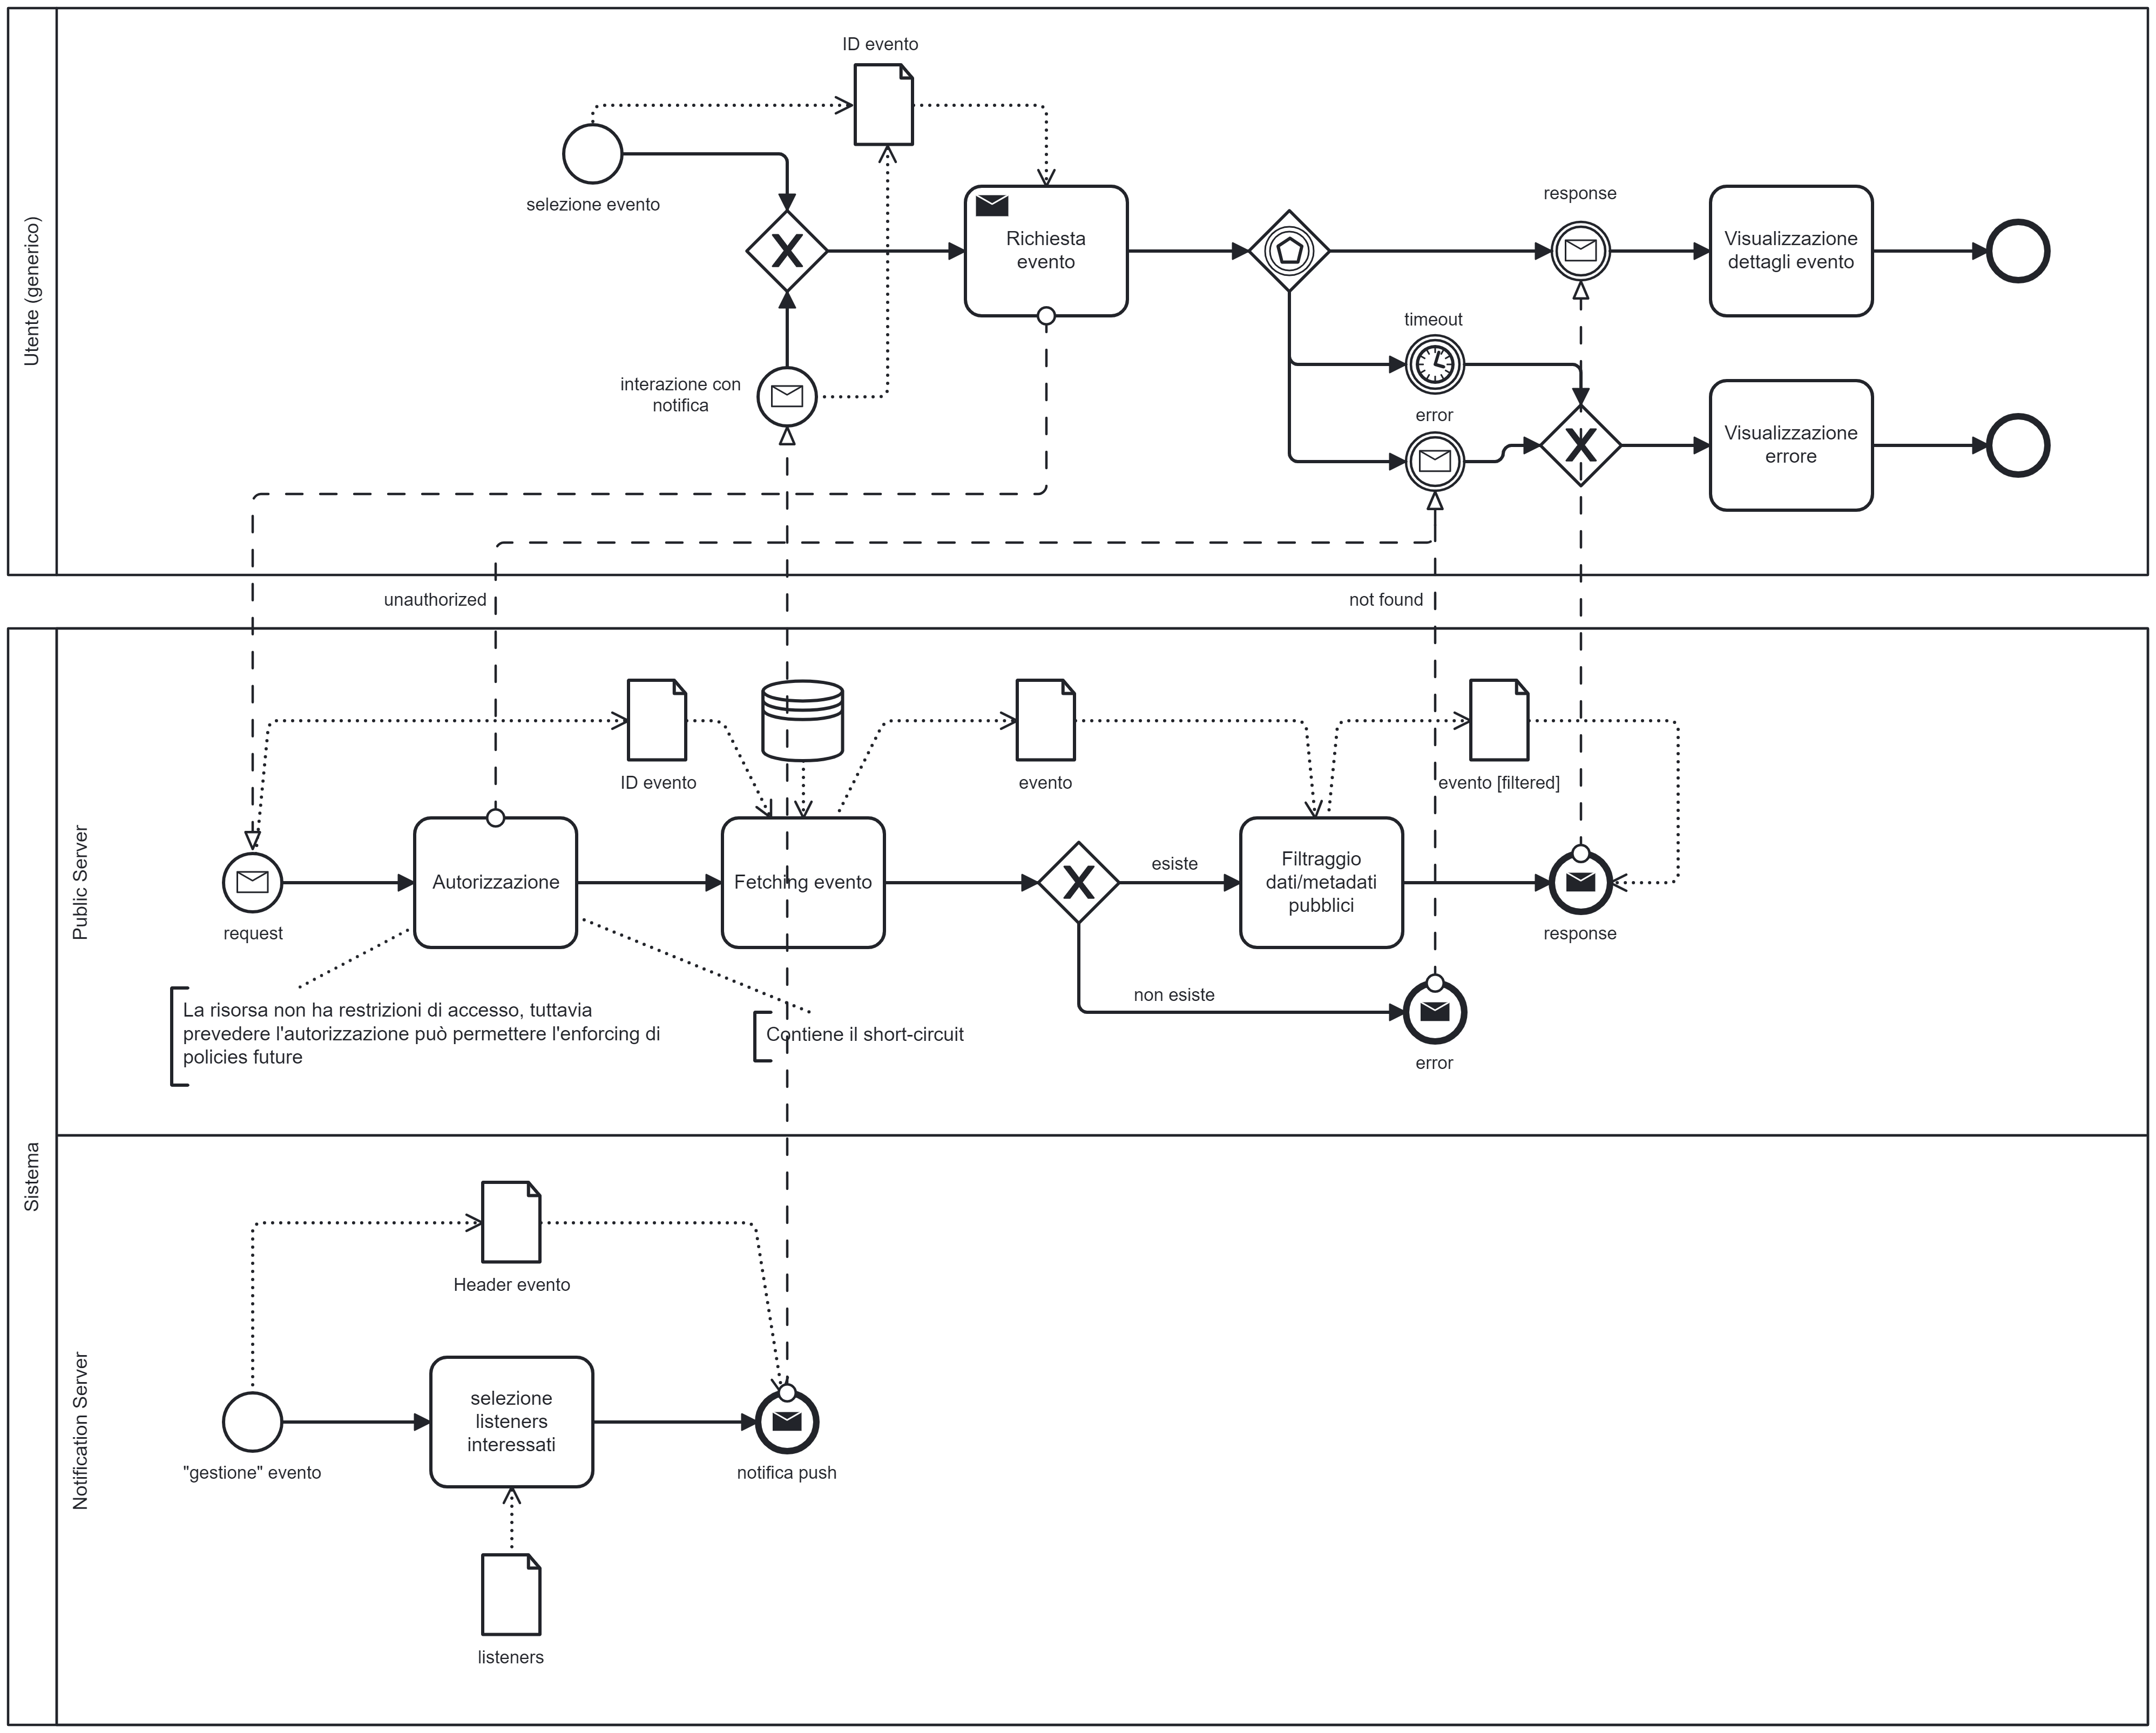
\includegraphics[width=1\textwidth]{Images/BPMN - details.png}
    \caption{Grafo BPMN per la visualizzazione dei dettagli di un evento}
\end{figure}

\clearpage

\subsubsection{Definizione categorie}
\index{Definizione categorie}

\begin{figure}[htbp]
    \label{7.1.5}
    \centering
    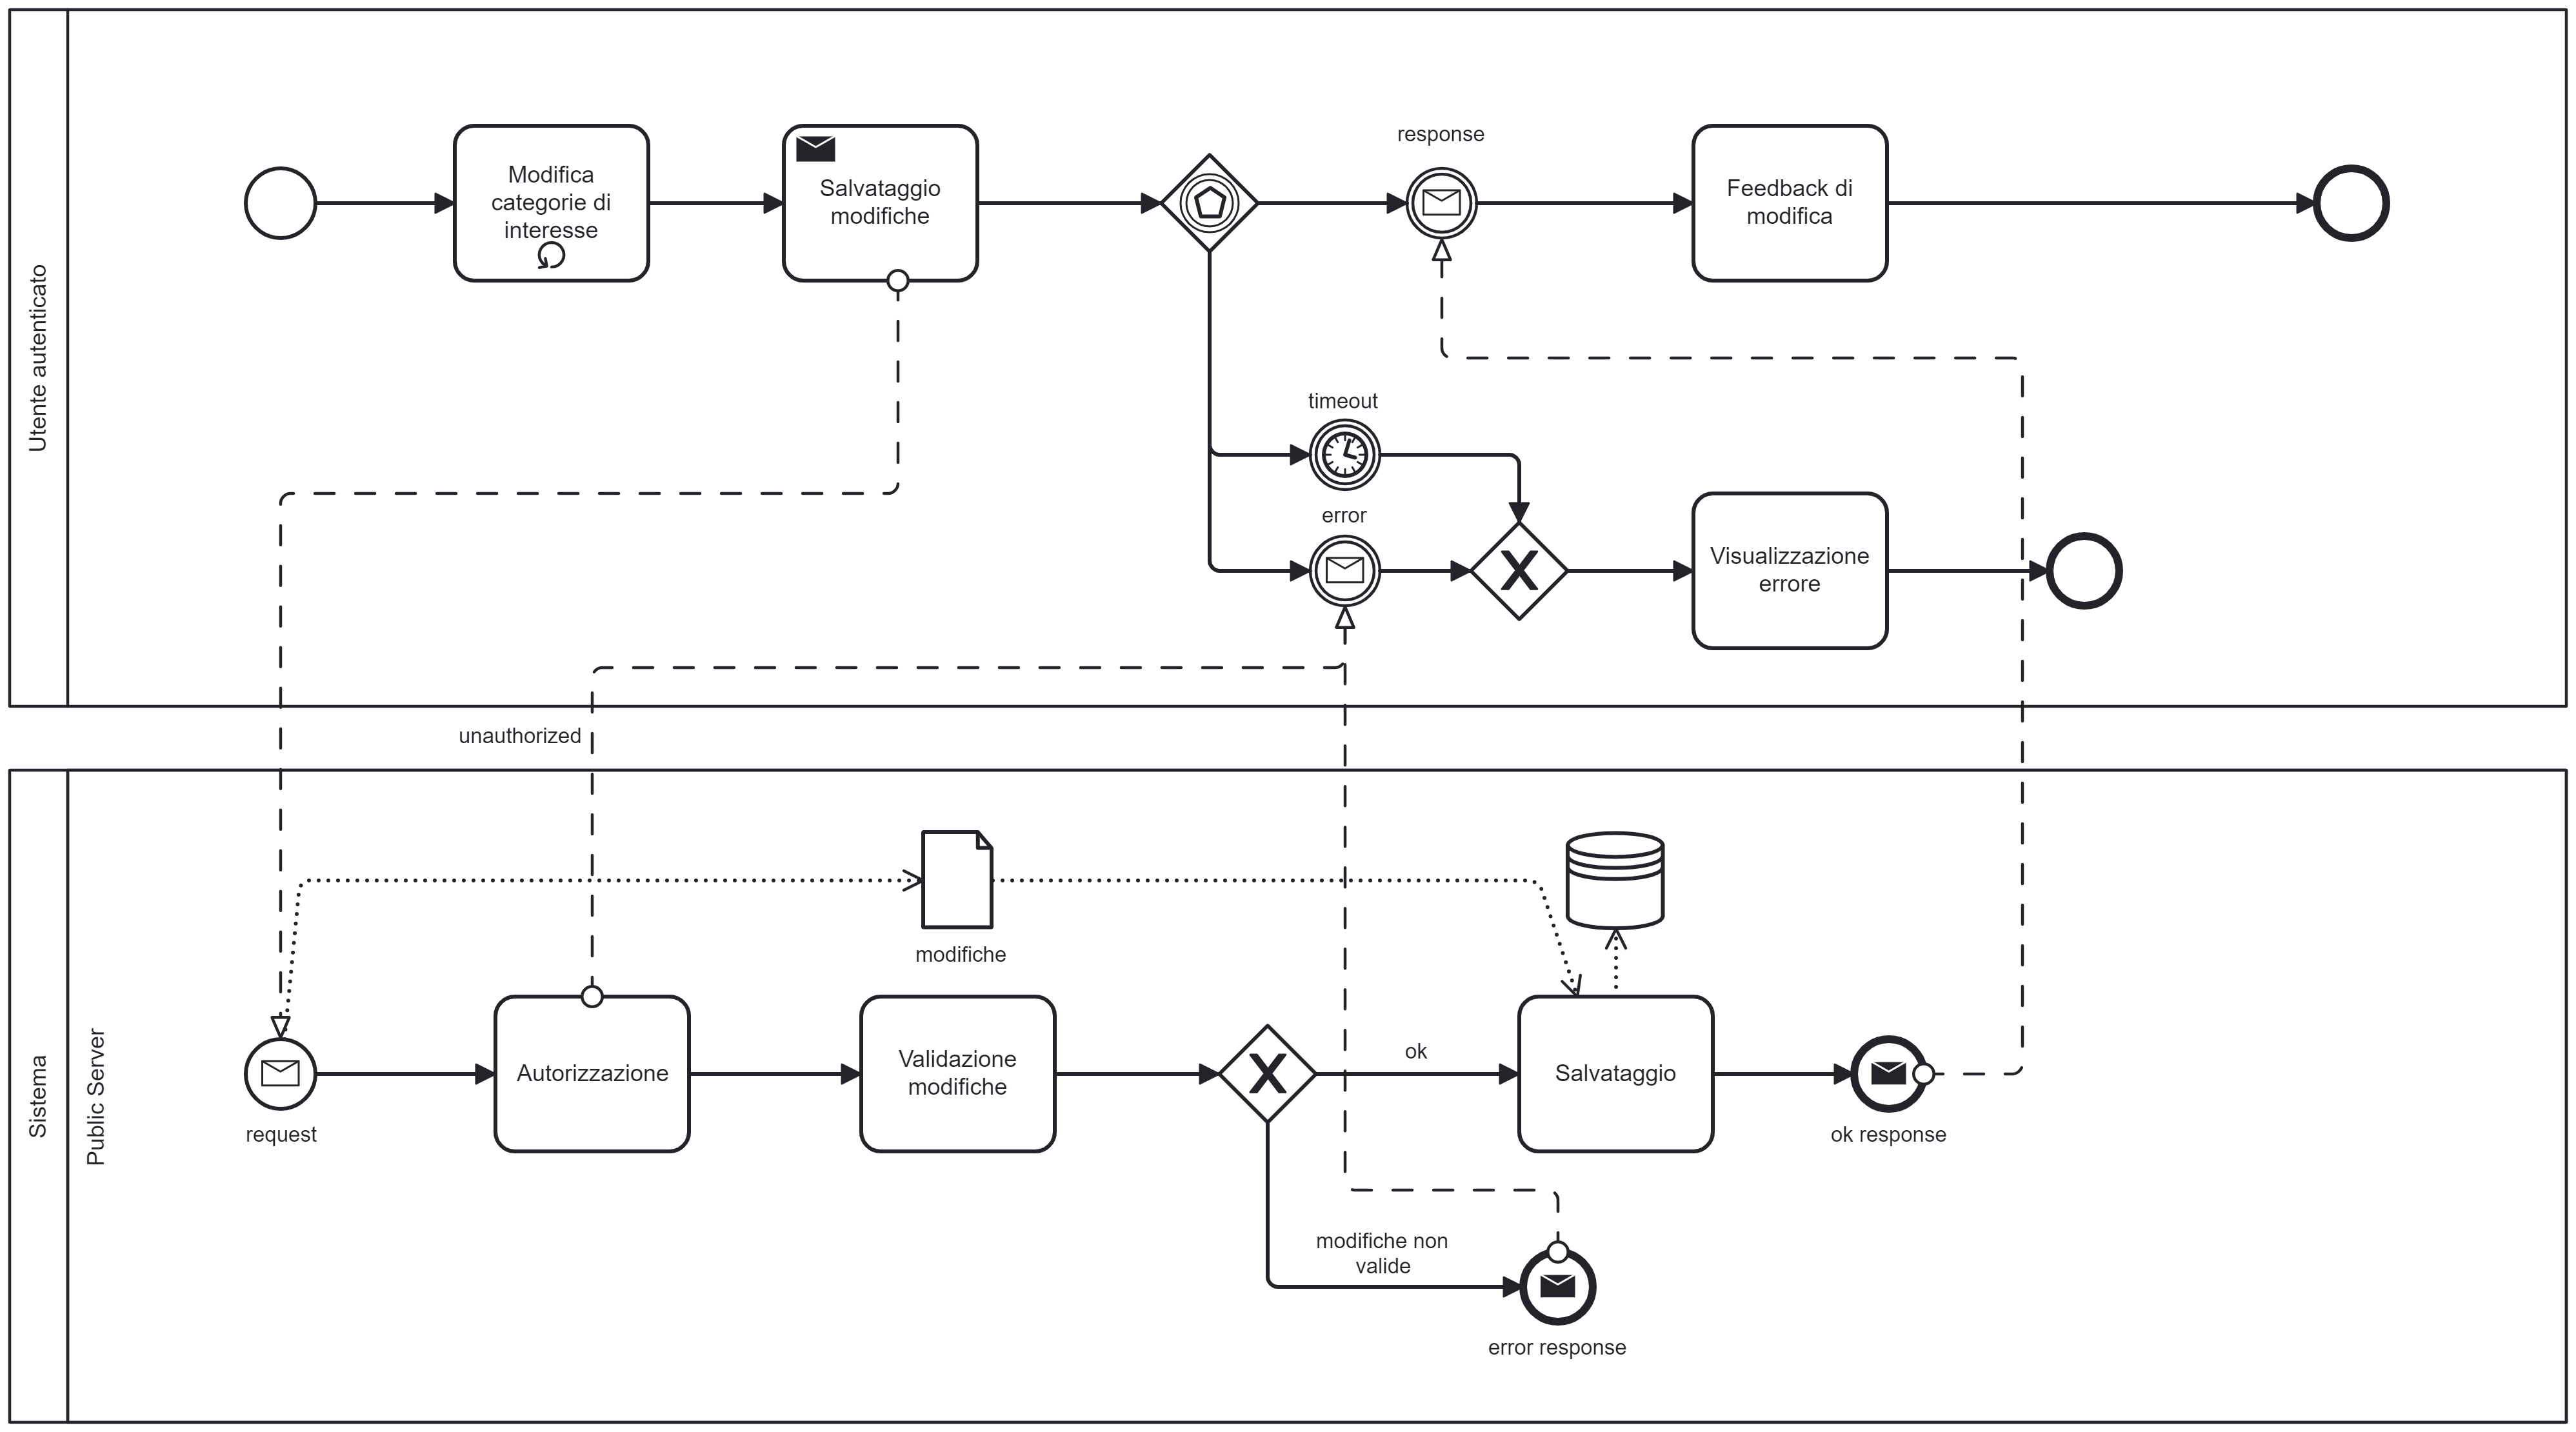
\includegraphics[width=1\textwidth]{Images/BPMN - categories.png}
    \caption{Grafo BPMN per la definizione delle categorie degli eventi}
\end{figure}

\clearpage

\subsubsection{Definizione zone di interesse}
\index{Definizione zone di interesse}

\begin{figure}[htbp]
    \label{7.1.6}
    \centering
    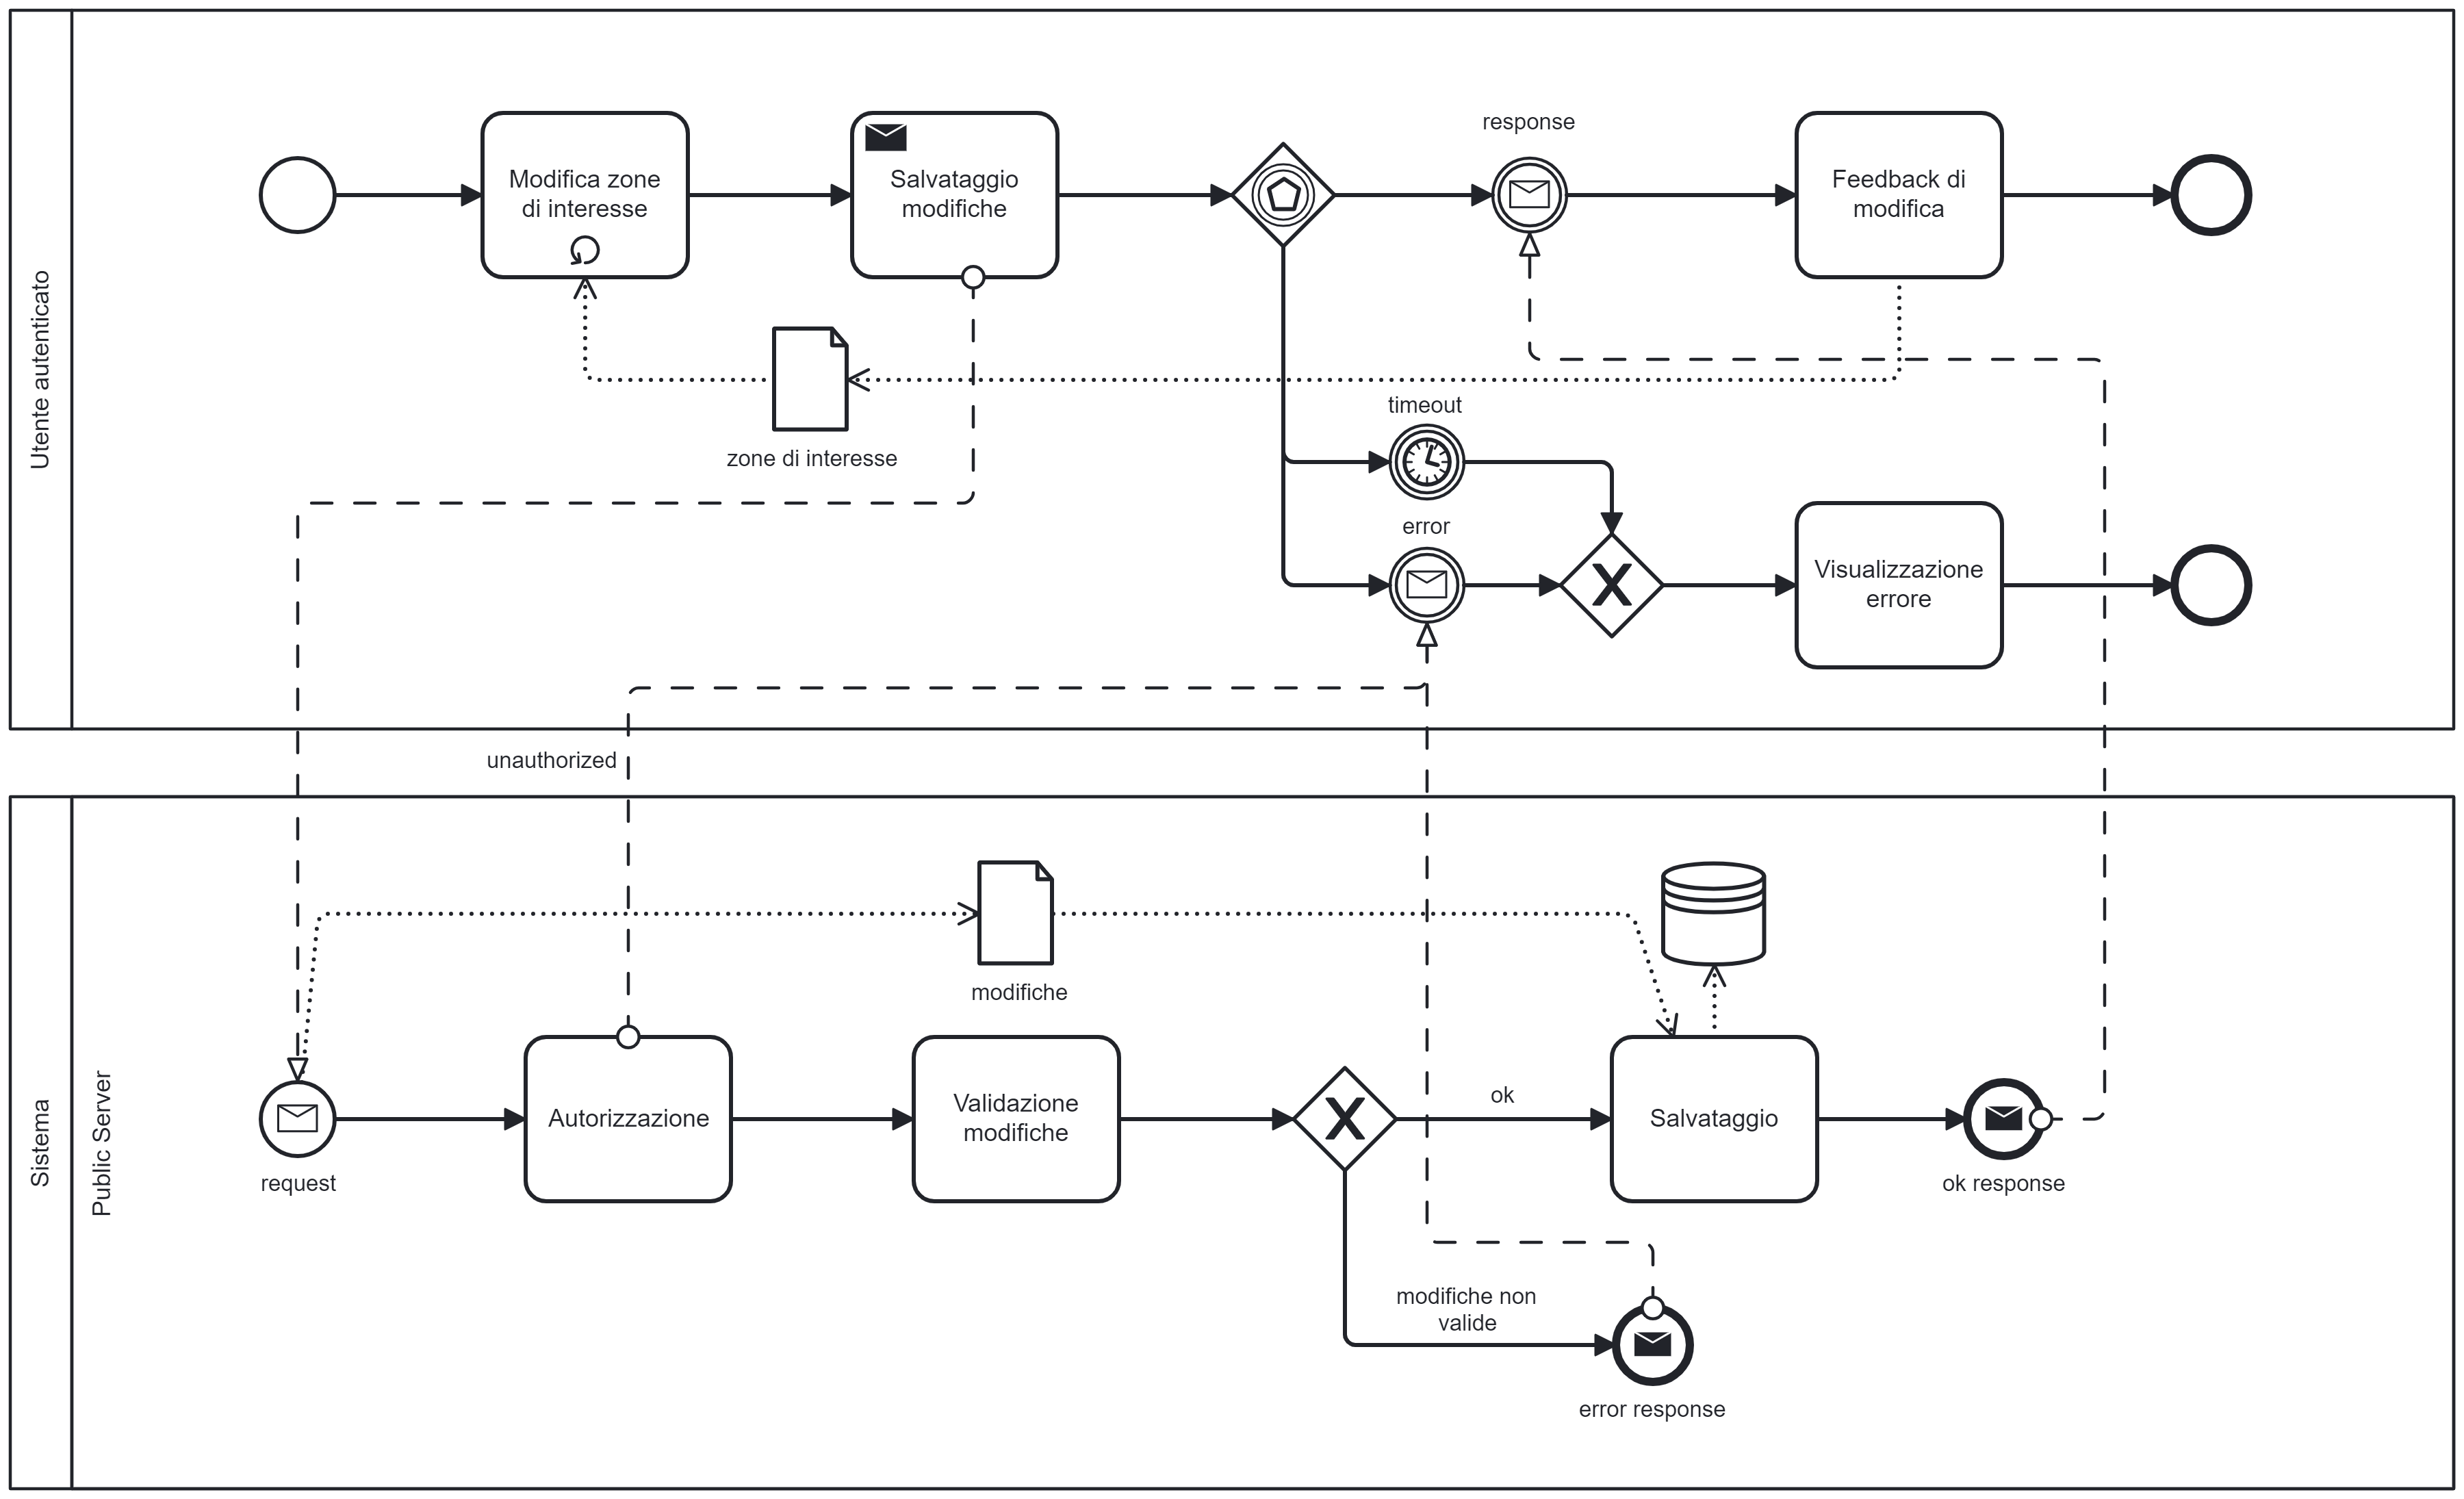
\includegraphics[width=1\textwidth]{Images/BPMN - zone.png}
    \caption{Grafo BPMN per la definizione delle zone di interesse}
\end{figure}
\clearpage

\subsection{Utente desktop}
\index{Utente desktop}

\subsubsection{Definizione sottocategorie}
\index{Definizione sottocategorie}

\begin{figure}[htbp]
    \label{7.2.1}
    \centering
    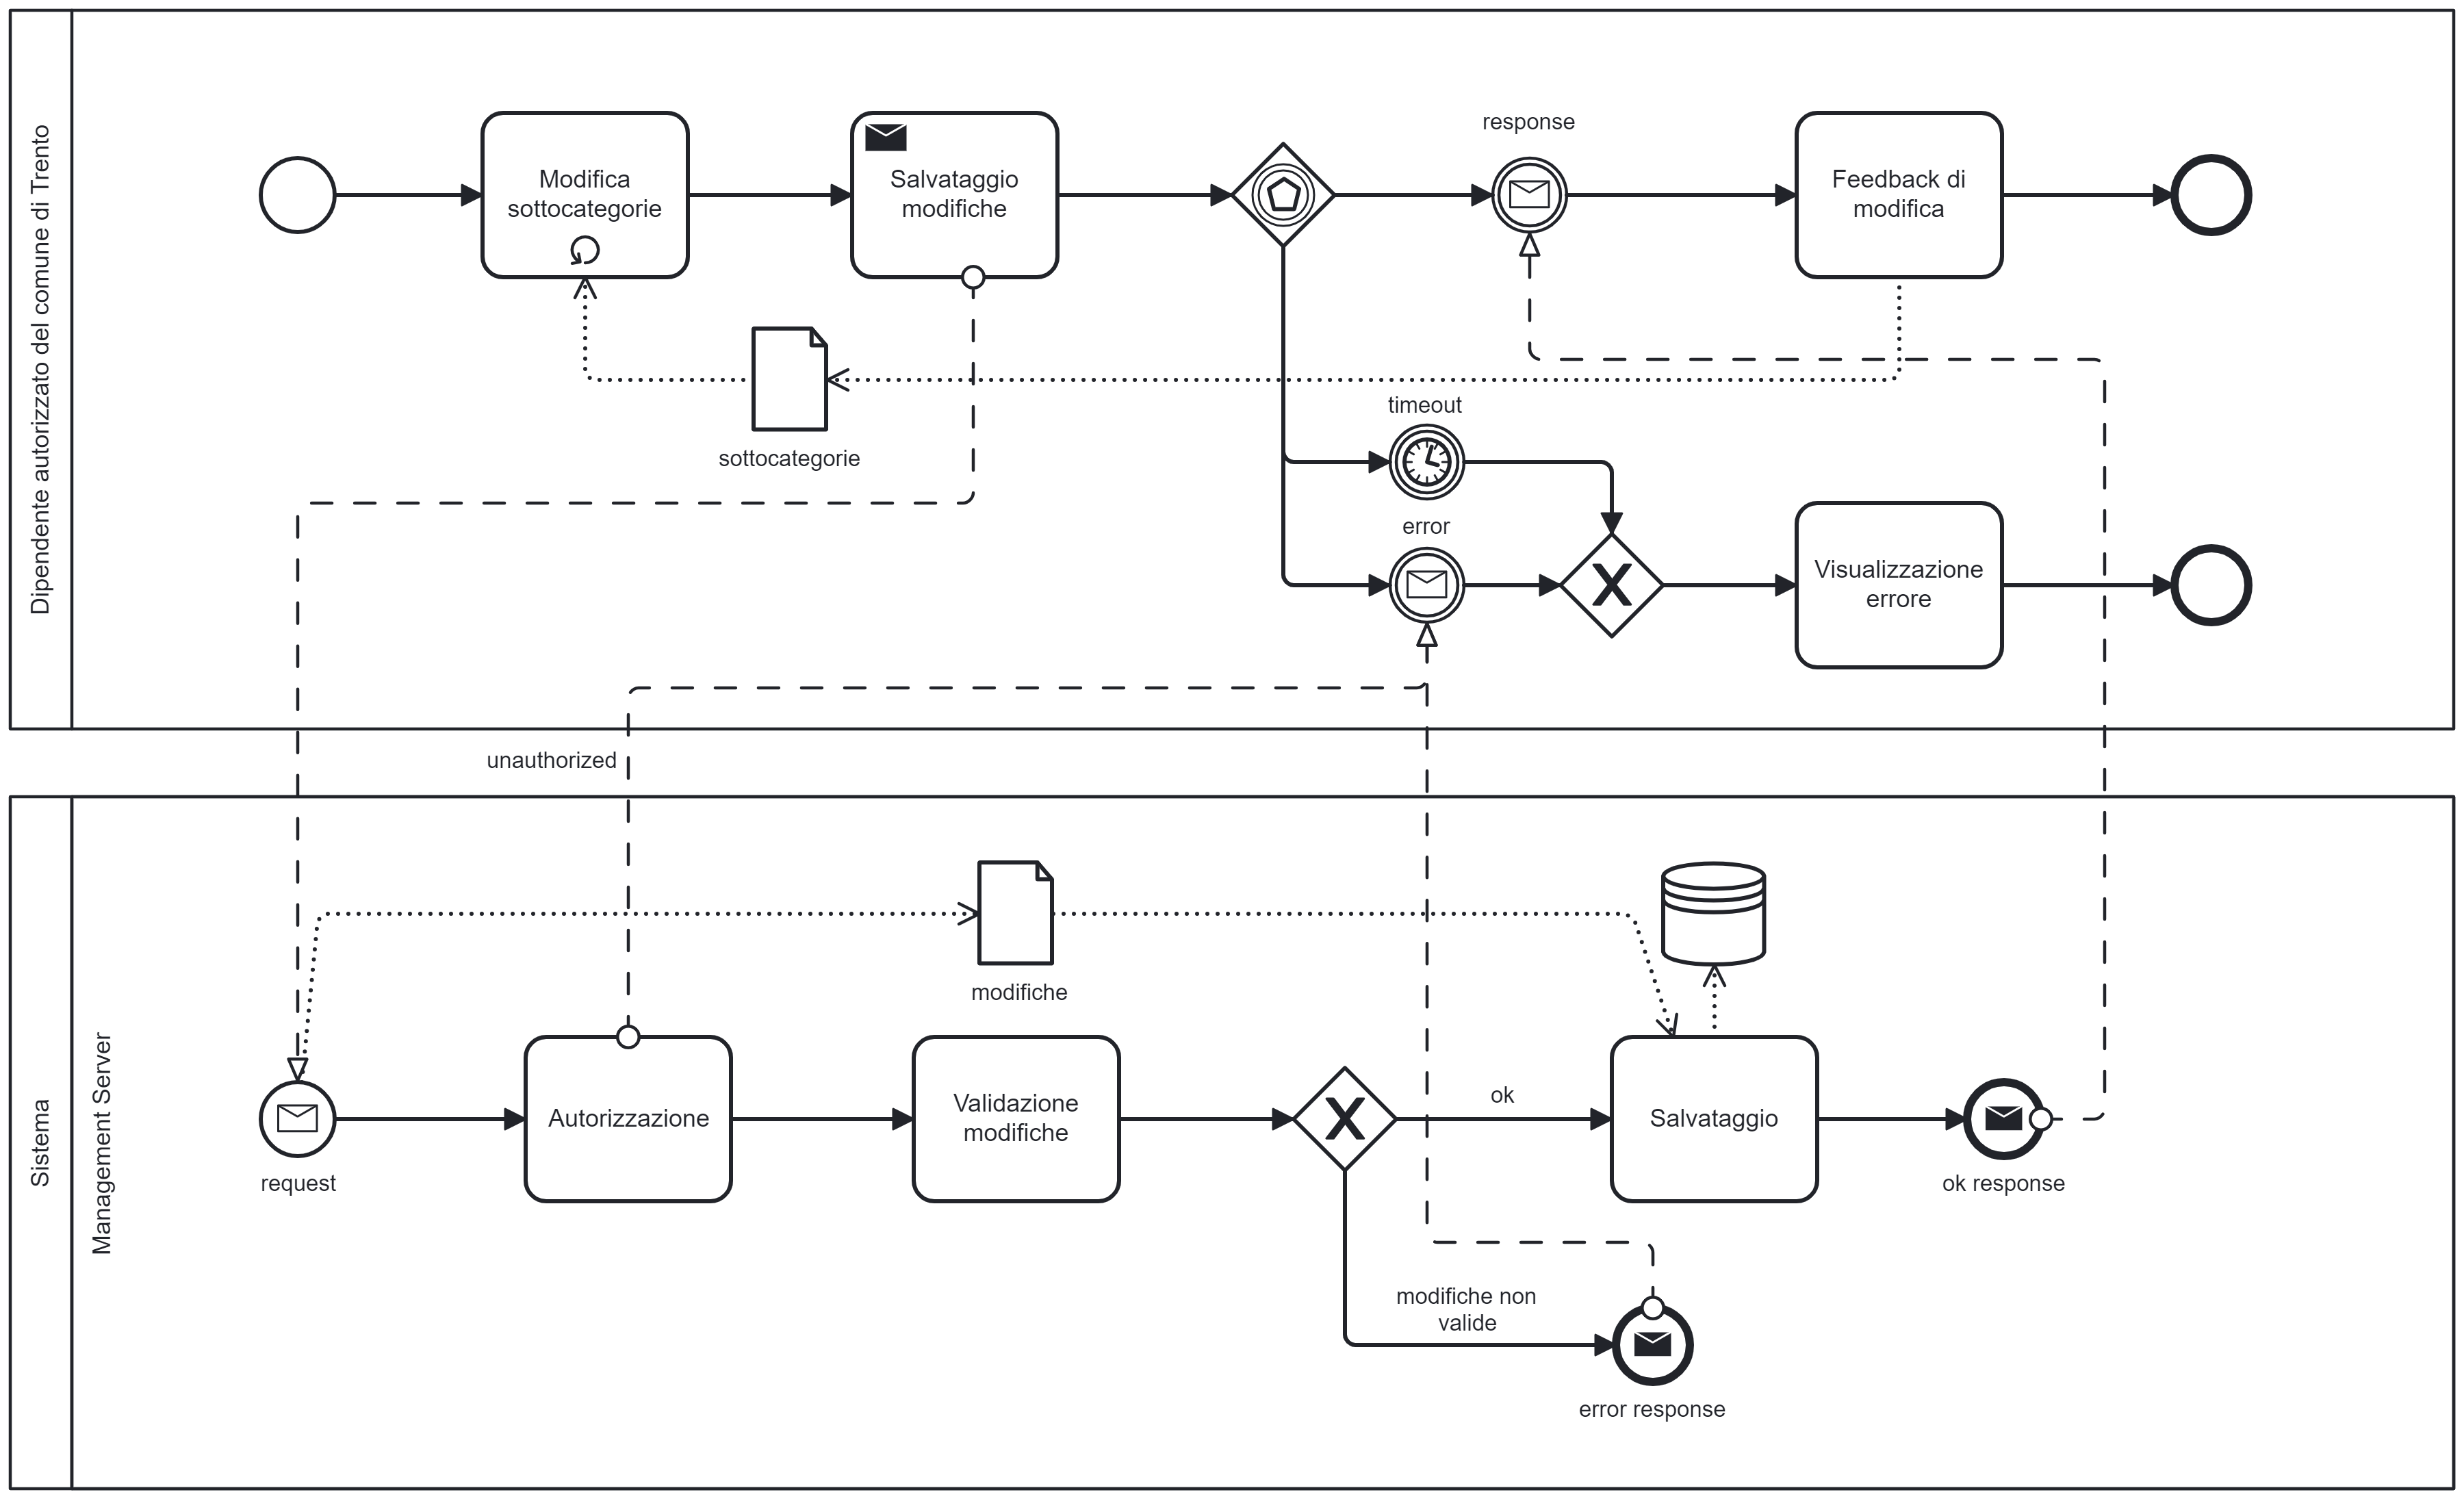
\includegraphics[width=1\textwidth]{Images/BPMN - sottocategorie.png}
    \caption{Grafo BPMN per la definizione delle sottocategorie}
\end{figure}
\clearpage

\subsubsection{Visualizzazione storico degli eventi pubblicati}
\index{Visualizzazione storico degli eventi pubblicati}

\begin{figure}[htbp]
    \label{7.2.2}
    \centering
    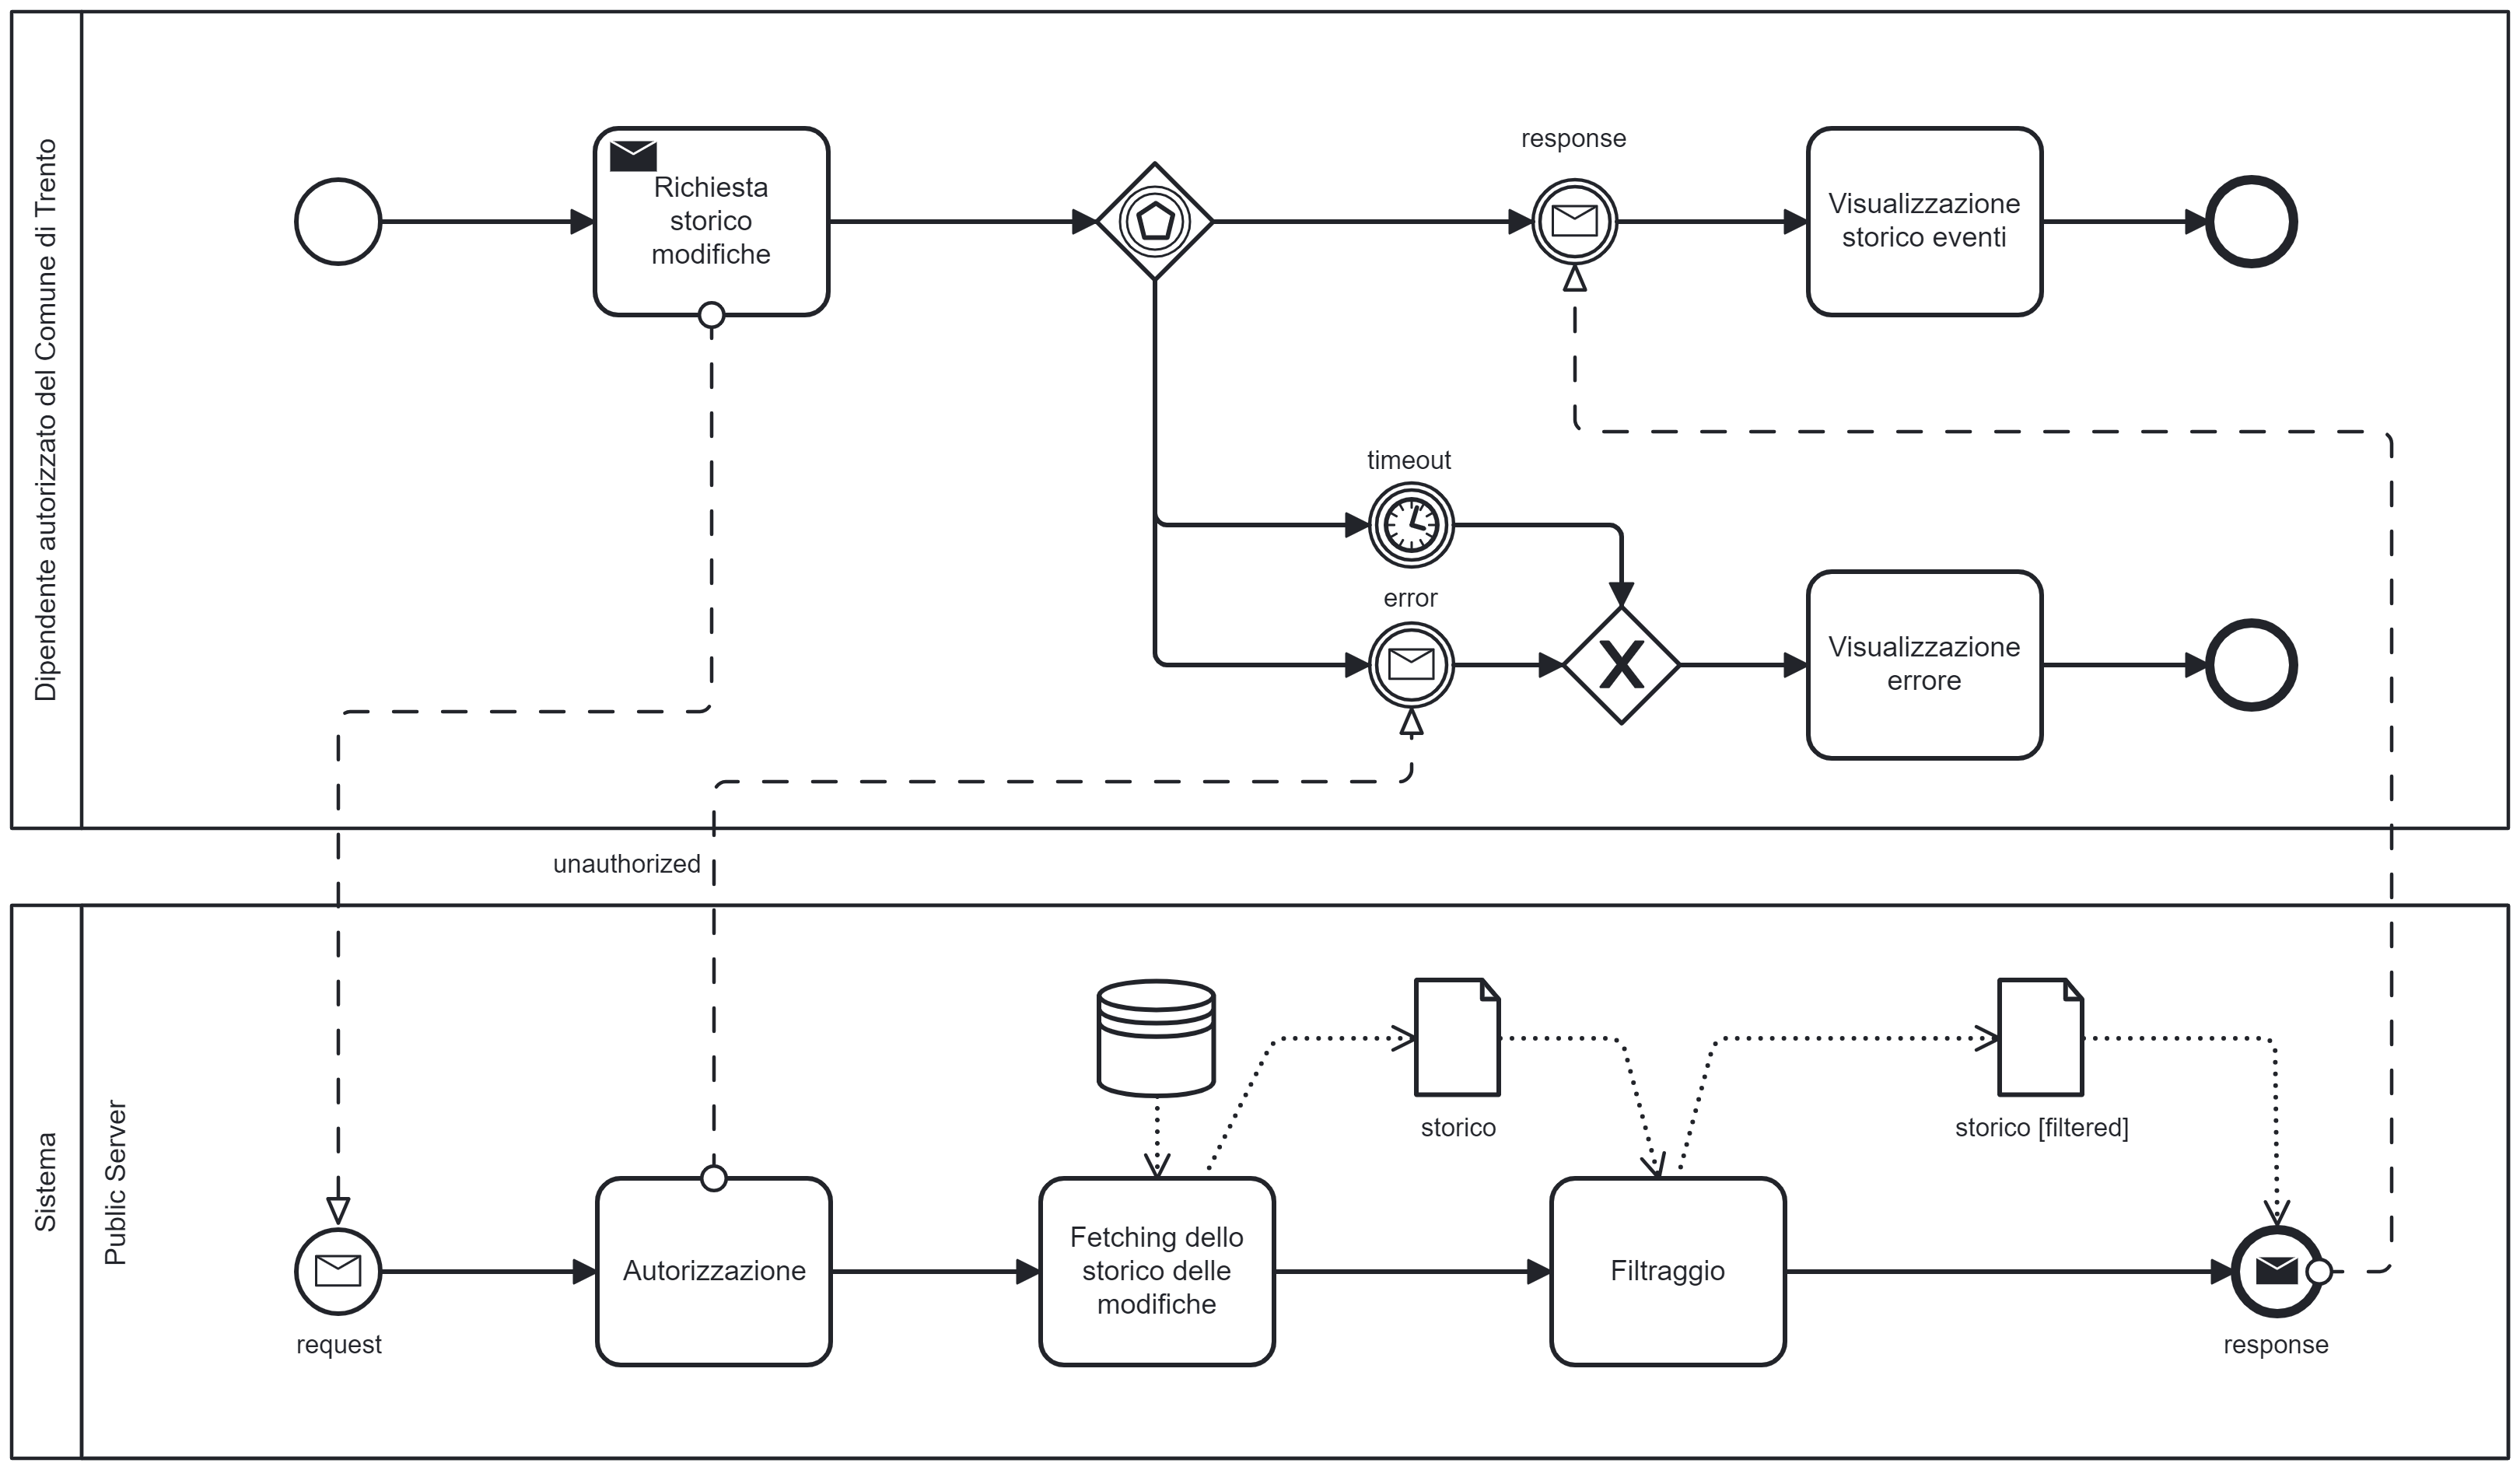
\includegraphics[width=1\textwidth]{Images/BPMN - storico.png}
    \caption{Grafo BPMN per la visualizzazione dello storico degli eventi pubblicati}
\end{figure}
\clearpage

\subsubsection{Gestione eventi}
\index{Gestione eventi}

\begin{figure}[htbp]
    \label{7.2.3}
    \centering
    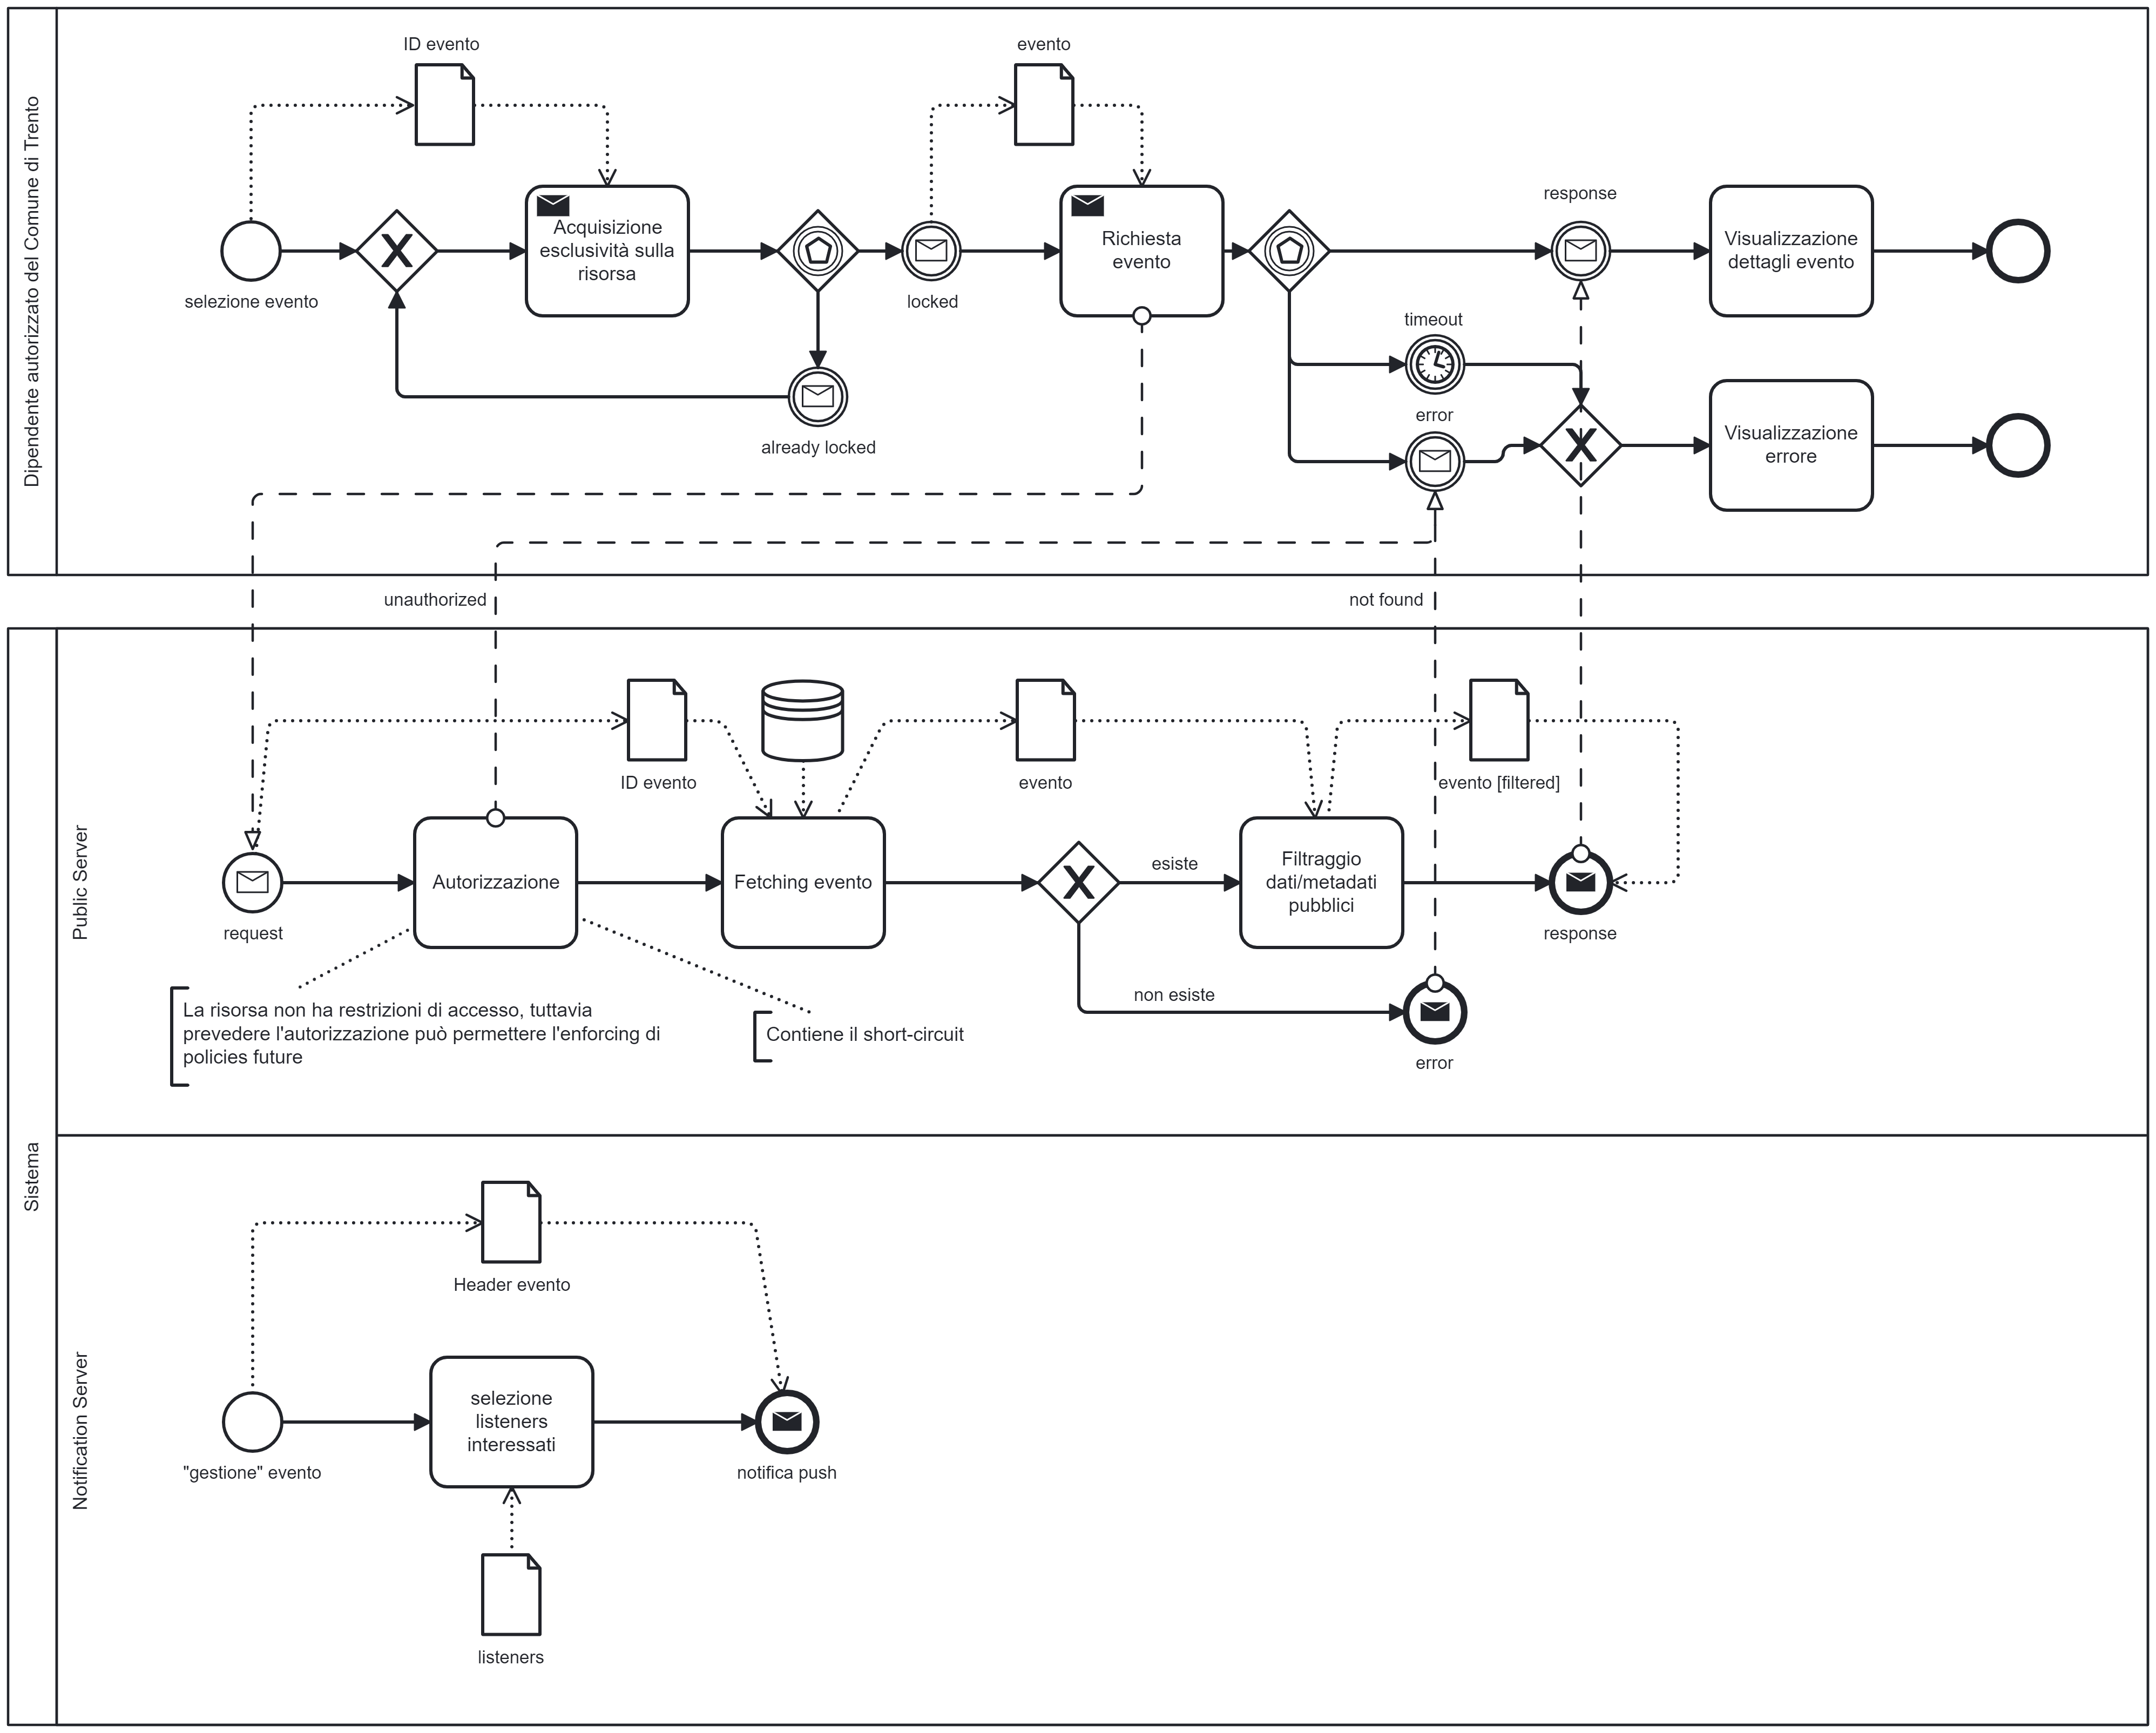
\includegraphics[width=1\textwidth]{Images/BPMN - gestione_evento.png}
    \caption{Grafo BPMN per la gestione degli eventi}
\end{figure}

\clearpage

\section{Casi d'uso}
\index{Casi d'uso} % Aggiunge una voce all'indice

\subsection{Utente anonimo}
\index{Utente anonimo}

\subsubsection{Registrazione ed autenticazione dell' utente anonimo}
\index{Registrazione ed autenticazione dell' utente anonimo}

\begin{table}[htbp]
    \label{8.1.1}
    \centering
    \begin{tabularx}{\textwidth}{| l | p{0.795\textwidth} |}
        \Xhline{2pt} % Linea spessa
        Nome caso d'uso & Autenticazione o registrazione di un utente anonimo \\
        \Xhline{2pt} % Linea spessa
        ID & 001 \\
        \hline
        Descrizione & L'utente accede con un account precedentemente creato all'interno del sistema, oppure ne crea uno nuovo \\
        \hline
        Attori primari & Utente anonimo \\
        \hline
        Attori secondari & Server di autenticazione \\
        \hline
        Precondizioni & Nessuna \\
        \hline
        Flusso principale & 
        \begin{enumerate}[topsep=5pt,partopsep=0pt,parsep=0pt,itemsep=0pt,before=\vspace{-\baselineskip},after=\vspace{-\baselineskip}]                
            \item L'utente apre l'applicativo mobile
            \item L'utente seleziona l'opzione d'accesso
            \item Il sistema reindirizza l'utente al servizio di autenticazione esterno
            \item Se l'utente non è ancora registrato:
            \begin{enumerate}[leftmargin=*, nosep]
                \item L'utente crea un profilo
                \item Vengono sincronizzate le preferenze utente
            \end{enumerate}
            \item Se l'utente è già registrato:
            \begin{enumerate}[leftmargin=*, nosep]
            	\item L'utente si autentica
            \end{enumerate}
            \item l'utente anonimo diventa un utente autenticato
        \end{enumerate}
        \\
        \hline
        Flusso alternativo & 
        Se la registrazione non va a buon fine:
        \begin{enumerate}[topsep=12pt,partopsep=0pt,parsep=0pt,itemsep=0pt,before=\vspace{-\baselineskip},after=\vspace{-\baselineskip}]
            \item L'utente rimane anonimo.
        \end{enumerate}
        \\
        \hline
    \end{tabularx}
    \caption{Registrazione ed autenticazione dell' utente anonimo}
    \label{tab:tabella_use_case001}
\end{table}

\clearpage

\subsection{Utente anonimo o autenticato}
\index{Utente anonimo o autenticato}

\subsubsection{Visualizzazione degli eventi}
\index{Visualizzazione degli eventi}

\begin{table}[htbp]
    \label{8.2.1}
    \centering
    \begin{tabularx}{\textwidth}{| l | p{0.795\textwidth} |}
        \Xhline{2pt} % Linea spessa
        Nome caso d'uso & Visualizzazione degli eventi \\
        \Xhline{2pt} % Linea spessa
        ID & 002 \\
        \hline
        Descrizione & L'utente intende visualizzare gli eventi disponibili\\
        \hline
        Attori primari & Utente anonimo o autenticato\\
        \hline
        Attori secondari &  Nessuno \\
        \hline
        Precondizioni & Nessuna \\
        \hline
        Flusso principale & 
        \begin{enumerate}[topsep=5pt,partopsep=0pt,parsep=0pt,itemsep=0pt,before=\vspace{-\baselineskip},after=\vspace{-\baselineskip}]                
            \item L'utente apre l'applicativo mobile
            \item L'applicativo mobile mostra la lista degli eventi
        \end{enumerate}
        \\
        \hline
        Flusso alternativo & 
        Se non vi è connettività internet
        \begin{enumerate}[topsep=10pt,partopsep=0pt,parsep=0pt,itemsep=0pt,before=\vspace{-\baselineskip},after=\vspace{-\baselineskip}]                
            \item Viene mostrato un banner che indica la mancanza di connessione
        \end{enumerate}
        \\
        \hline
    \end{tabularx}
    \caption{Visualizzazione degli eventi}
    \label{tab:tabella_use_case002}
\end{table}

\subsubsection{Visualizzazione dei dettagli di un evento}
\index{Visualizzazione dei dettagli di un evento}

\begin{table}[htbp]
    \label{8.2.2}
    \centering
    \begin{tabularx}{\textwidth}{| l | X |}
        \Xhline{2pt} % Linea spessa
        Nome caso d'uso & Visualizzazione dei dettagli di un evento\\
        \Xhline{2pt} % Linea spessa
        ID & 003 \\
        \hline
        Descrizione & L'utente intende visualizzare i dettagli di un evento specifico\\
        \hline
        Attori primari & Utente anonimo o autenticato\\
        \hline
        Attori secondari & Nessuno \\
        \hline
        Precondizioni & Nessuna (Flusso n.2), l'utente ha ricevuto una notifica push riguardo ad un evento (Flusso n.1)\\
        \hline
        Flusso n.1 & 
        \begin{enumerate}[topsep=5pt,partopsep=0pt,parsep=0pt,itemsep=0pt,before=\vspace{-\baselineskip},after=\vspace{-\baselineskip}] 
            \item L'utente clicca la notifica
            \item Viene automaticamente aperta l'applicazione mobile
            \item Vene automaticamente visualizzata la schermata dei dettagli
        \end{enumerate}
        \\
        \hline
        Flusso n.2 & 
        \begin{enumerate}[topsep=5pt,partopsep=0pt,parsep=0pt,itemsep=0pt,before=\vspace{-\baselineskip},after=\vspace{-\baselineskip}]                
            \item L'utente apre l'applicativo mobile
            \item L'utente clicca un evento della lista
            \item Viene visualizzata la schermata dei dettagli di tale evento
        \end{enumerate}
        \\
        \hline
    \end{tabularx}
    \caption{Visualizzazione dei dettagli di un evento}
\end{table}

\clearpage

\subsubsection{Filtraggio degli eventi}
\index{Filtraggio degli eventi}

\begin{table}[htbp]
    \label{8.2.3}
    \centering
    \begin{tabularx}{\textwidth}{| l | X |}
        \Xhline{2pt} % Linea spessa
        Nome caso d'uso & Filtraggio degli eventi \\
        \Xhline{2pt} % Linea spessa
        ID & 004 \\
        \hline
        Descrizione & L'utente intende nascondere alcuni elementi dalla lista\\
        \hline
        Attori primari & Utente anonimo o autenticato\\
        \hline
        Attori secondari & Nessuno \\
        \hline
        Precondizioni & Nessuna \\
        \hline
        Flusso n.1 &
        \begin{enumerate}[topsep=5pt,partopsep=0pt,parsep=0pt,itemsep=0pt,before=\vspace{-\baselineskip},after=\vspace{-\baselineskip}]                
            \item L'utente apre l'applicativo mobile
            \item L'utente interagisce con un evento della lista, effettuando la procedura per nasconderlo
            \item L'evento non appare più nella lista degli eventi
        \end{enumerate}
        \\
        \hline
        Flusso n.2 &
        \begin{enumerate}[topsep=5pt,partopsep=0pt,parsep=0pt,itemsep=0pt,before=\vspace{-\baselineskip},after=\vspace{-\baselineskip}]                
            \item Viene aperto l'applicativo mobile
            \item Sono aperte le impostazioni
            \item L'utente seleziona le categorie di suo interesse su cui continuare a ricevere informazioni per eventi futuri
        \end{enumerate}
        \\
        \hline
        Postcondizioni & Tutti gli eventi futuri verranno filtrati in funzione delle categorie impostate dall'utente nel flusso n.2\\
        \hline
    \end{tabularx}
    \caption{Filtraggio degli eventi}
\end{table}

\subsubsection{Selezione dei percorsi e aree di interesse}
\index{Selezione dei percorsi di interesse}

\begin{table}[htbp]
    \label{8.2.4}
    \centering
    \begin{tabularx}{\textwidth}{| l | p{0.795\textwidth} |}
        \Xhline{2pt} % Linea spessa
        Nome caso d'uso & Selezione dei percorsi e aree di interesse \\
        \Xhline{2pt} % Linea spessa
        ID & 005 \\
        \hline
        Descrizione & L'utente indica i percorsi di suo interesse\\
        \hline
        Attori primari & Utente anonimo o autenticato\\
        \hline
        Attori secondari & Nessuno \\
        \hline
        Precondizioni & Nessuna \\
        \hline
        Flusso principale & 
        \begin{enumerate}[topsep=5pt,partopsep=0pt,parsep=0pt,itemsep=0pt,before=\vspace{-\baselineskip},after=\vspace{-\baselineskip}]                
            \item L'utente apre l'applicazione mobile
            \item L'utente entra nella sezione dedicata alle aree e percorsi d'interesse
            \item L'utente crea in modalità interattiva il percorso o l'area d'interesse
            \item L'utente salva l'area o il percorso d'interesse appena creato
        \end{enumerate}
        \\
        \hline
    \end{tabularx}
    \caption{Selezione dei percorsi di interesse}
    \label{tab:tabella_use_case004}
\end{table}

\clearpage


\subsection{Dipendente autorizzato del Comune di Trento}
\index{Dipendente autorizzato del Comune di Trento}

\subsubsection{Creazione sottocategorie}
\index{Definizione delle sottocategorie}

\begin{table}[htbp]
    \label{8.3.1}
    \centering
    \begin{tabularx}{\textwidth}{| l | p{0.795\textwidth} |}
        \Xhline{2pt} % Linea spessa
        Nome caso d'uso & Gestione sottocategorie \\
        \Xhline{2pt} % Linea spessa
        ID & 005 \\
        \hline
        Descrizione & Il dipendente autorizzato del Comune di Trento (D.A.) intende gestire le sottocategorie per eventi di sua competenza\\
        \hline
        Attori primari & Dipendente autorizzato del Comune di Trento\\
        \hline
        Attori secondari & Nessuno \\
        \hline
        Precondizioni & Nessuna \\
        \hline
        Flusso principale & 
        \begin{enumerate}[topsep=5pt,partopsep=0pt,parsep=0pt,itemsep=0pt,before=\vspace{-\baselineskip},after=\vspace{-\baselineskip}]                
            \item Il D.A. apre l'applicativo desktop
            \item Il D.A. si autentica
            \item Il D.A. entra nella sezione dedicata alla gestione delle sottocategorie
            \item Il D.A. crea, modifica o elimina una sottocategoria
            \item Il sistema memorizza la creazione, la modifica o l'eliminazione della sottocategoria
        \end{enumerate}
        \\
        \hline
        Flusso secondario & 
        Se la creazione non va a buon fine:
        \begin{enumerate}[topsep=10pt,partopsep=0pt,parsep=0pt,itemsep=0pt,before=\vspace{-\baselineskip},after=\vspace{-\baselineskip}]                
            \item Il D.A. sarà avvisato dell'errore
        \end{enumerate}
        \\
        \hline
    \end{tabularx}
    \caption{Definizione delle sottocategorie}
    \label{tab:tabella_use_case006}
\end{table}

\clearpage

\subsubsection{Creazione degli eventi}
\index{Creazione degli eventi}

\begin{table}[htbp]
    \label{8.3.2}
    \centering
    \begin{tabularx}{\textwidth}{| l | p{0.795\textwidth} |}
        \Xhline{2pt} % Linea spessa
        Nome caso d'uso & Creazione degli eventi \\
        \Xhline{2pt} % Linea spessa
        ID & 006 \\
        \hline
        Descrizione & Il dipendente autorizzato del Comune di Trento crea un evento di sua competenza\\
        \hline
        Attori primari & Dipendente autorizzato del Comune di Trento\\
        \hline
        Attori secondari & Nessuno, oppure tutti o alcuni utenti \\
        \hline
        Precondizioni & Nessuna \\
        \hline
        Flusso principale & 
        \begin{enumerate}[topsep=5pt,partopsep=0pt,parsep=0pt,itemsep=0pt,before=\vspace{-\baselineskip},after=\vspace{-\baselineskip}]                
            \item Il dipendente autorizzato (D.A.) apre l'applicativo desktop
            \item Il D.A. si autentica
            \item Il D.A. entra nella sezione dedicata alla creazione di un nuovo evento
            \item Il D.A. compila tutti i campi che caratterizzano il nuovo evento
            \item Il D.A. pubblica l'evento
            \item Tutti gli utenti che hanno le notifiche attivate per quel tipo di eventi riceveranno una notifica
        \end{enumerate}
        \\
        \hline
        Flusso secondario & 
        Se la creazione non va a buon fine:
        \begin{enumerate}[topsep=10pt,partopsep=0pt,parsep=0pt,itemsep=0pt,before=\vspace{-\baselineskip},after=\vspace{-\baselineskip}]                
            \item Il D.A. verrà avvisato dell'errore
        \end{enumerate}
        \\
        \hline
    \end{tabularx}
    \caption{Creazione nuovi eventi}
    \label{tab:tabella_use_case006}
\end{table}

\clearpage

\subsubsection{Modifica di un evento}
\index{Modifica di un evento}

\begin{table}[htbp]
    \label{8.3.3}
    \centering
    \begin{tabularx}{\textwidth}{| l | p{0.795\textwidth} |}
        \Xhline{2pt} % Linea spessa
        Nome caso d'uso & Modifica di un evento \\
        \Xhline{2pt} % Linea spessa
        ID & 007 \\
        \hline
        Descrizione & Il dipendente autorizzato del Comune di Trento (D.A.) intende modificare uno o più campi di un evento\\
        \hline
        Attori primari & Dipendente autorizzato del Comune di Trento\\
        \hline
        Attori secondari & Nessuno, oppure tutti o alcuni utenti  \\
        \hline
        Precondizioni & Il D.A. ha i permessi sufficienti per modificare l'evento, l'evento è di sua competenza\\
        \hline
        Flusso principale & 
        \begin{enumerate}[topsep=5pt,partopsep=0pt,parsep=0pt,itemsep=0pt,before=\vspace{-\baselineskip},after=\vspace{-\baselineskip}]                
            \item Il D.A. apre l'applicativo desktop
            \item Il D.A. si autentica
            \item Il D.A. entra nella sezione dedicata alla modifica degli memorizzati sul sistema
            \item Il D.A. modificati i campi che intende aggiornare
            \item Il D.A. pubblica la modifica
            \item Il sistema memorizza l'evento
            \item Tutti gli utenti che hanno le notifiche attivate per quel tipo di modifiche, e quel tipo di eventi, riceveranno una notifica
        \end{enumerate}
        \\
        \hline
        Flusso secondario & 
        Se la modifica non va a buon fine
        \begin{enumerate}[topsep=10pt,partopsep=0pt,parsep=0pt,itemsep=0pt,before=\vspace{-\baselineskip},after=\vspace{-\baselineskip}]                
            \item Il D.A. verrà avvisato dell'errore
        \end{enumerate}
        \\
        \hline
    \end{tabularx}
    \caption{Modifica di un evento}
    \label{tab:tabella_use_case007}
\end{table}

\clearpage

\subsubsection{Eliminazione di un evento}
\index{Eliminzione di un evento}

\begin{table}[htbp]
    \label{8.3.4}
    \centering
    \begin{tabularx}{\textwidth}{| l | p{0.795\textwidth} |}
        \Xhline{2pt} % Linea spessa
        Nome caso d'uso & Eliminazione di un evento \\
        \Xhline{2pt} % Linea spessa
        ID & 008 \\
        \hline
        Descrizione & Il dipendente autorizzato del Comune di Trento (D.A.) intende eliminare un evento\\
        \hline
        Attori primari & Dipendente autorizzato del Comune di trento\\
        \hline
        Attori secondari & Nessuno \\
        \hline
        Precondizioni & Il D.A. ha i permessi sufficienti per eliminare l'evento e l'evento è di sua competenza \\
        \hline
        Flusso principale & 
        \begin{enumerate}[topsep=5pt,partopsep=0pt,parsep=0pt,itemsep=0pt,before=\vspace{-\baselineskip},after=\vspace{-\baselineskip}]                
            \item Il D.A. apre l'applicativo desktop
            \item Il D.A. si autentica
            \item Il D.A. entra nella sezione dedicata alla modifica degli eventi memorizzato sul sistema
            \item Il D.A. indica di voler eliminare un evento
            \item Il D.A. conferma di voler eliminare l'evento
            \item Il sistema elimina l'evento
            \item Il D.A. viene avvisato della corretta eliminazione
        \end{enumerate}
        \\
        \hline
        Flusso secondario & 
        Se la cancellazione non va a buon fine:
        \begin{enumerate}[topsep=10pt,partopsep=0pt,parsep=0pt,itemsep=0pt,before=\vspace{-\baselineskip},after=\vspace{-\baselineskip}]
            \item Il D.A. verrà avvisato dell'errore
        \end{enumerate}
        \\
        \hline
    \end{tabularx}
    \caption{Eliminazione di un evento}
    \label{tab:tabella_use_case008}
\end{table}

\clearpage

\section{Diagramma dei casi d'uso}
\index{Diagramma dei casi d'uso} % Aggiunge una voce all'indice

\subsection{Utente mobile}
\index{Utente mobile}

\begin{figure}[htbp]
    \centering
    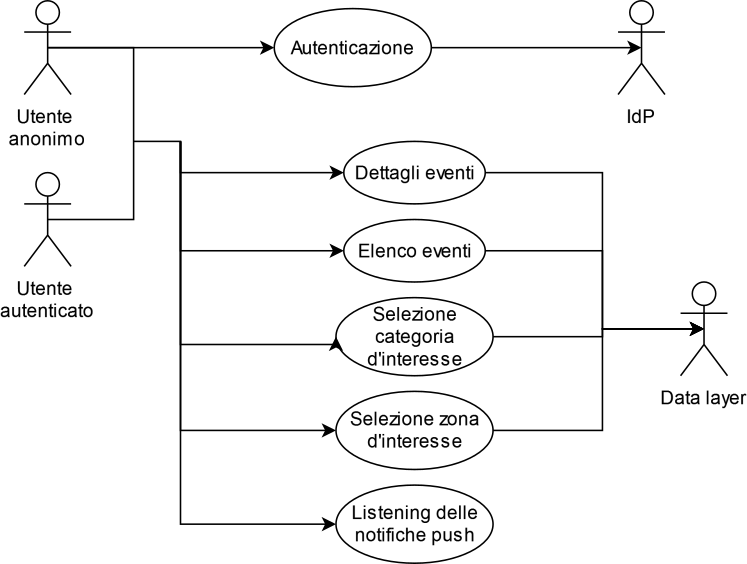
\includegraphics[width=0.75\textwidth]{Images/UseCase_Diagram - Utenti.png}
    \caption{Diagramma dei casi d'uso per gli utenti}
\end{figure}
\clearpage

\subsection{Utente desktop}
\index{Utente desktop}

\begin{figure}[htbp]
    \centering
    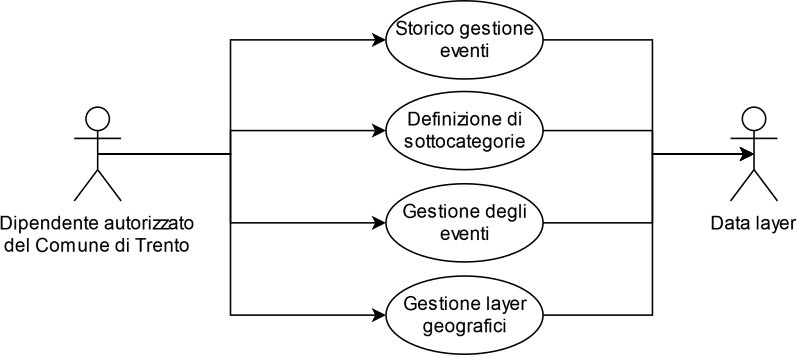
\includegraphics[width=0.75\textwidth]{Images/UseCase_Diagram - Comune.png}
    \caption{Diagramma dei casi d'uso per il dipendente del Comune di Trento}
\end{figure}

\subsection{Amministratore}
\index{Amministratore}

\begin{figure}[htbp]
    \centering
    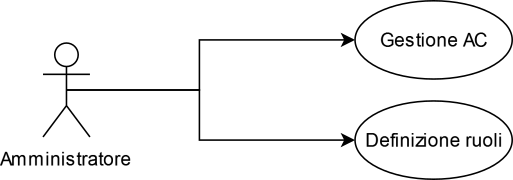
\includegraphics[width=0.5\textwidth]{Images/UseCase_Diagram - Amministratore.png}
    \caption{Diagramma dei casi d'uso per l'amministratore}
\end{figure}
\clearpage

\section{Resoconto}
\index{Resoconto} % Aggiunge una voce all'indice

Seguono le tabelle dei riferimenti per ambiente considerato, utili alla comprensione generale delle diverse sezioni riguardanti lo specifico obiettivo.\\

\subsection{Applicativo mobile}
\index{Applicativo mobile}

\begin{table}[htbp]
    \centering
    \begin{tabularx}{\textwidth}{|X|X|X|X|X|X|}
        \Xhline{2pt} % Linea spessa
        Obiettivo & Attore & Casi d'uso & Requisiti\newline funzionali & BPMN & Mockup \\
        \Xhline{2pt} % Linea spessa
        Visualizzazione degli eventi & \ref{3.1.1}\newline\ref{3.1.2} & \ref{8.2.1}\newline\ref{8.2.2} & \ref{5.1.1} & \ref{7.1.3}\newline{7.1.4} & \ref{4.1.1}\newline\ref{4.1.2} \\
        \hline
        Gestione\newline degli eventi significativi & \ref{3.1.3}\newline\ref{3.2.1} & \ref{8.2.3} & \ref{5.1.2}\newline\ref{5.1.3}\newline\ref{5.1.7} & \ref{7.1.5} & - \\
        \hline
        Gestione aree degli eventi significativi & \ref{3.1.1}\newline\ref{3.1.2} & - & \ref{5.1.8}\newline\ref{5.1.9} & \ref{7.1.6} & - \\
        \hline
        Visualizzazione spaziale degli \newline eventi & \ref{3.1.1}\newline\ref{3.1.2} & \ref{8.2.4}\newline\ref{8.2.5} & \ref{5.1.4} & - & - \\
        \hline
        Registrazione e accesso & \ref{3.1.1}\newline\ref{3.1.2} & \ref{8.1.1} & \ref{5.1.5}\newline\ref{5.1.6}\newline\ref{5.2.1} & \ref{7.1.1}\newline\ref{7.1.2} & - \\
        \hline
        Accesso alle notifiche & \ref{3.1.1}\newline\ref{3.1.2} & - & \ref{5.1.10} & - & \ref{4.1.3} \\
        \hline
    \end{tabularx}
    \caption{Tabella riassuntiva}
    \label{tab:tabellaMobile}
\end{table}

\subsection{Applicativo desktop}
\index{Applicativo desktop}

\begin{table}[htbp]
    \centering
    \begin{tabularx}{\textwidth}{|X|X|X|X|X|X|}
        \Xhline{2pt} % Linea spessa
        Obiettivo & Attore & Casi d'uso & Requisiti\newline funzionali & BPMN & Mockup \\
        \Xhline{2pt} % Linea spessa
        Gestione eventi di competenza & \ref{3.1.3}\newline\ref{3.2.1} & \ref{8.3.1}\newline\ref{8.3.2}\newline\ref{8.3.3}\newline\ref{8.3.4} & \ref{5.3.2}\newline\ref{5.3.1}\newline\ref{5.3.3}\newline\ref{5.3.6}\newline\ref{5.3.7}\newline\ref{5.3.8}\newline\ref{5.3.9}\newline\ref{5.3.10} & \ref{7.2.1}\newline\ref{7.2.2} & \ref{4.2} \\
        \hline
        Gestione eventi di altri & \ref{3.1.3}\newline\ref{3.2.1} & - & \ref{5.3.4}\newline\ref{5.3.5} & \ref{7.2.2} & -\\
        \hline
    \end{tabularx}
    \caption{Tabella riassuntiva}
    \label{tab:TabellaDesktop}
\end{table}

\clearpage

\subsection{Amministrazione di sistema}
\index{Amministrazione di sistema}

\begin{table}[htbp]
    \centering
    \begin{tabularx}{\textwidth}{|X|X|X|X|X|X|}
        \Xhline{2pt} % Linea spessa
        Obiettivo & Attore & Casi d'uso & Requisiti\newline funzionali & BPMN & Mockup \\
        \Xhline{2pt} % Linea spessa
        Management degli utenti & \ref{3.1.4} & - & \ref{5.5.1}\newline\ref{5.5.2}\newline\ref{5.5.3}\newline\ref{5.5.4} & \ref{7.2.3} & - \\
        \hline
    \end{tabularx}
    \caption{Tabella riassuntiva}
    \label{tab:TabellaAmministrazione}
\end{table}

\end{document}